\documentclass[11pt]{article}

    \usepackage[breakable]{tcolorbox}
    \usepackage{parskip} % Stop auto-indenting (to mimic markdown behaviour)
    
    \usepackage{iftex}
    \ifPDFTeX
    	\usepackage[T1]{fontenc}
    	\usepackage{mathpazo}
    \else
    	\usepackage{fontspec}
    \fi

    % Basic figure setup, for now with no caption control since it's done
    % automatically by Pandoc (which extracts ![](path) syntax from Markdown).
    \usepackage{graphicx}
    % Maintain compatibility with old templates. Remove in nbconvert 6.0
    \let\Oldincludegraphics\includegraphics
    % Ensure that by default, figures have no caption (until we provide a
    % proper Figure object with a Caption API and a way to capture that
    % in the conversion process - todo).
    \usepackage{caption}
    \DeclareCaptionFormat{nocaption}{}
    \captionsetup{format=nocaption,aboveskip=0pt,belowskip=0pt}

    \usepackage{float}
    \floatplacement{figure}{H} % forces figures to be placed at the correct location
    \usepackage{xcolor} % Allow colors to be defined
    \usepackage{enumerate} % Needed for markdown enumerations to work
    \usepackage{geometry} % Used to adjust the document margins
    \usepackage{amsmath} % Equations
    \usepackage{amssymb} % Equations
    \usepackage{textcomp} % defines textquotesingle
    % Hack from http://tex.stackexchange.com/a/47451/13684:
    \AtBeginDocument{%
        \def\PYZsq{\textquotesingle}% Upright quotes in Pygmentized code
    }
    \usepackage{upquote} % Upright quotes for verbatim code
    \usepackage{eurosym} % defines \euro
    \usepackage[mathletters]{ucs} % Extended unicode (utf-8) support
    \usepackage{fancyvrb} % verbatim replacement that allows latex
    \usepackage{grffile} % extends the file name processing of package graphics 
                         % to support a larger range
    \makeatletter % fix for old versions of grffile with XeLaTeX
    \@ifpackagelater{grffile}{2019/11/01}
    {
      % Do nothing on new versions
    }
    {
      \def\Gread@@xetex#1{%
        \IfFileExists{"\Gin@base".bb}%
        {\Gread@eps{\Gin@base.bb}}%
        {\Gread@@xetex@aux#1}%
      }
    }
    \makeatother
    \usepackage[Export]{adjustbox} % Used to constrain images to a maximum size
    \adjustboxset{max size={0.9\linewidth}{0.9\paperheight}}

    % The hyperref package gives us a pdf with properly built
    % internal navigation ('pdf bookmarks' for the table of contents,
    % internal cross-reference links, web links for URLs, etc.)
    \usepackage{hyperref}
    % The default LaTeX title has an obnoxious amount of whitespace. By default,
    % titling removes some of it. It also provides customization options.
    \usepackage{titling}
    \usepackage{longtable} % longtable support required by pandoc >1.10
    \usepackage{booktabs}  % table support for pandoc > 1.12.2
    \usepackage[inline]{enumitem} % IRkernel/repr support (it uses the enumerate* environment)
    \usepackage[normalem]{ulem} % ulem is needed to support strikethroughs (\sout)
                                % normalem makes italics be italics, not underlines
    \usepackage{mathrsfs}
    

    
    % Colors for the hyperref package
    \definecolor{urlcolor}{rgb}{0,.145,.698}
    \definecolor{linkcolor}{rgb}{.71,0.21,0.01}
    \definecolor{citecolor}{rgb}{.12,.54,.11}

    % ANSI colors
    \definecolor{ansi-black}{HTML}{3E424D}
    \definecolor{ansi-black-intense}{HTML}{282C36}
    \definecolor{ansi-red}{HTML}{E75C58}
    \definecolor{ansi-red-intense}{HTML}{B22B31}
    \definecolor{ansi-green}{HTML}{00A250}
    \definecolor{ansi-green-intense}{HTML}{007427}
    \definecolor{ansi-yellow}{HTML}{DDB62B}
    \definecolor{ansi-yellow-intense}{HTML}{B27D12}
    \definecolor{ansi-blue}{HTML}{208FFB}
    \definecolor{ansi-blue-intense}{HTML}{0065CA}
    \definecolor{ansi-magenta}{HTML}{D160C4}
    \definecolor{ansi-magenta-intense}{HTML}{A03196}
    \definecolor{ansi-cyan}{HTML}{60C6C8}
    \definecolor{ansi-cyan-intense}{HTML}{258F8F}
    \definecolor{ansi-white}{HTML}{C5C1B4}
    \definecolor{ansi-white-intense}{HTML}{A1A6B2}
    \definecolor{ansi-default-inverse-fg}{HTML}{FFFFFF}
    \definecolor{ansi-default-inverse-bg}{HTML}{000000}

    % common color for the border for error outputs.
    \definecolor{outerrorbackground}{HTML}{FFDFDF}

    % commands and environments needed by pandoc snippets
    % extracted from the output of `pandoc -s`
    \providecommand{\tightlist}{%
      \setlength{\itemsep}{0pt}\setlength{\parskip}{0pt}}
    \DefineVerbatimEnvironment{Highlighting}{Verbatim}{commandchars=\\\{\}}
    % Add ',fontsize=\small' for more characters per line
    \newenvironment{Shaded}{}{}
    \newcommand{\KeywordTok}[1]{\textcolor[rgb]{0.00,0.44,0.13}{\textbf{{#1}}}}
    \newcommand{\DataTypeTok}[1]{\textcolor[rgb]{0.56,0.13,0.00}{{#1}}}
    \newcommand{\DecValTok}[1]{\textcolor[rgb]{0.25,0.63,0.44}{{#1}}}
    \newcommand{\BaseNTok}[1]{\textcolor[rgb]{0.25,0.63,0.44}{{#1}}}
    \newcommand{\FloatTok}[1]{\textcolor[rgb]{0.25,0.63,0.44}{{#1}}}
    \newcommand{\CharTok}[1]{\textcolor[rgb]{0.25,0.44,0.63}{{#1}}}
    \newcommand{\StringTok}[1]{\textcolor[rgb]{0.25,0.44,0.63}{{#1}}}
    \newcommand{\CommentTok}[1]{\textcolor[rgb]{0.38,0.63,0.69}{\textit{{#1}}}}
    \newcommand{\OtherTok}[1]{\textcolor[rgb]{0.00,0.44,0.13}{{#1}}}
    \newcommand{\AlertTok}[1]{\textcolor[rgb]{1.00,0.00,0.00}{\textbf{{#1}}}}
    \newcommand{\FunctionTok}[1]{\textcolor[rgb]{0.02,0.16,0.49}{{#1}}}
    \newcommand{\RegionMarkerTok}[1]{{#1}}
    \newcommand{\ErrorTok}[1]{\textcolor[rgb]{1.00,0.00,0.00}{\textbf{{#1}}}}
    \newcommand{\NormalTok}[1]{{#1}}
    
    % Additional commands for more recent versions of Pandoc
    \newcommand{\ConstantTok}[1]{\textcolor[rgb]{0.53,0.00,0.00}{{#1}}}
    \newcommand{\SpecialCharTok}[1]{\textcolor[rgb]{0.25,0.44,0.63}{{#1}}}
    \newcommand{\VerbatimStringTok}[1]{\textcolor[rgb]{0.25,0.44,0.63}{{#1}}}
    \newcommand{\SpecialStringTok}[1]{\textcolor[rgb]{0.73,0.40,0.53}{{#1}}}
    \newcommand{\ImportTok}[1]{{#1}}
    \newcommand{\DocumentationTok}[1]{\textcolor[rgb]{0.73,0.13,0.13}{\textit{{#1}}}}
    \newcommand{\AnnotationTok}[1]{\textcolor[rgb]{0.38,0.63,0.69}{\textbf{\textit{{#1}}}}}
    \newcommand{\CommentVarTok}[1]{\textcolor[rgb]{0.38,0.63,0.69}{\textbf{\textit{{#1}}}}}
    \newcommand{\VariableTok}[1]{\textcolor[rgb]{0.10,0.09,0.49}{{#1}}}
    \newcommand{\ControlFlowTok}[1]{\textcolor[rgb]{0.00,0.44,0.13}{\textbf{{#1}}}}
    \newcommand{\OperatorTok}[1]{\textcolor[rgb]{0.40,0.40,0.40}{{#1}}}
    \newcommand{\BuiltInTok}[1]{{#1}}
    \newcommand{\ExtensionTok}[1]{{#1}}
    \newcommand{\PreprocessorTok}[1]{\textcolor[rgb]{0.74,0.48,0.00}{{#1}}}
    \newcommand{\AttributeTok}[1]{\textcolor[rgb]{0.49,0.56,0.16}{{#1}}}
    \newcommand{\InformationTok}[1]{\textcolor[rgb]{0.38,0.63,0.69}{\textbf{\textit{{#1}}}}}
    \newcommand{\WarningTok}[1]{\textcolor[rgb]{0.38,0.63,0.69}{\textbf{\textit{{#1}}}}}
    
    
    % Define a nice break command that doesn't care if a line doesn't already
    % exist.
    \def\br{\hspace*{\fill} \\* }
    % Math Jax compatibility definitions
    \def\gt{>}
    \def\lt{<}
    \let\Oldtex\TeX
    \let\Oldlatex\LaTeX
    \renewcommand{\TeX}{\textrm{\Oldtex}}
    \renewcommand{\LaTeX}{\textrm{\Oldlatex}}
    % Document parameters
    % Document title
    \title{Conditionals}
    
    
    
    
    
% Pygments definitions
\makeatletter
\def\PY@reset{\let\PY@it=\relax \let\PY@bf=\relax%
    \let\PY@ul=\relax \let\PY@tc=\relax%
    \let\PY@bc=\relax \let\PY@ff=\relax}
\def\PY@tok#1{\csname PY@tok@#1\endcsname}
\def\PY@toks#1+{\ifx\relax#1\empty\else%
    \PY@tok{#1}\expandafter\PY@toks\fi}
\def\PY@do#1{\PY@bc{\PY@tc{\PY@ul{%
    \PY@it{\PY@bf{\PY@ff{#1}}}}}}}
\def\PY#1#2{\PY@reset\PY@toks#1+\relax+\PY@do{#2}}

\@namedef{PY@tok@w}{\def\PY@tc##1{\textcolor[rgb]{0.73,0.73,0.73}{##1}}}
\@namedef{PY@tok@c}{\let\PY@it=\textit\def\PY@tc##1{\textcolor[rgb]{0.25,0.50,0.50}{##1}}}
\@namedef{PY@tok@cp}{\def\PY@tc##1{\textcolor[rgb]{0.74,0.48,0.00}{##1}}}
\@namedef{PY@tok@k}{\let\PY@bf=\textbf\def\PY@tc##1{\textcolor[rgb]{0.00,0.50,0.00}{##1}}}
\@namedef{PY@tok@kp}{\def\PY@tc##1{\textcolor[rgb]{0.00,0.50,0.00}{##1}}}
\@namedef{PY@tok@kt}{\def\PY@tc##1{\textcolor[rgb]{0.69,0.00,0.25}{##1}}}
\@namedef{PY@tok@o}{\def\PY@tc##1{\textcolor[rgb]{0.40,0.40,0.40}{##1}}}
\@namedef{PY@tok@ow}{\let\PY@bf=\textbf\def\PY@tc##1{\textcolor[rgb]{0.67,0.13,1.00}{##1}}}
\@namedef{PY@tok@nb}{\def\PY@tc##1{\textcolor[rgb]{0.00,0.50,0.00}{##1}}}
\@namedef{PY@tok@nf}{\def\PY@tc##1{\textcolor[rgb]{0.00,0.00,1.00}{##1}}}
\@namedef{PY@tok@nc}{\let\PY@bf=\textbf\def\PY@tc##1{\textcolor[rgb]{0.00,0.00,1.00}{##1}}}
\@namedef{PY@tok@nn}{\let\PY@bf=\textbf\def\PY@tc##1{\textcolor[rgb]{0.00,0.00,1.00}{##1}}}
\@namedef{PY@tok@ne}{\let\PY@bf=\textbf\def\PY@tc##1{\textcolor[rgb]{0.82,0.25,0.23}{##1}}}
\@namedef{PY@tok@nv}{\def\PY@tc##1{\textcolor[rgb]{0.10,0.09,0.49}{##1}}}
\@namedef{PY@tok@no}{\def\PY@tc##1{\textcolor[rgb]{0.53,0.00,0.00}{##1}}}
\@namedef{PY@tok@nl}{\def\PY@tc##1{\textcolor[rgb]{0.63,0.63,0.00}{##1}}}
\@namedef{PY@tok@ni}{\let\PY@bf=\textbf\def\PY@tc##1{\textcolor[rgb]{0.60,0.60,0.60}{##1}}}
\@namedef{PY@tok@na}{\def\PY@tc##1{\textcolor[rgb]{0.49,0.56,0.16}{##1}}}
\@namedef{PY@tok@nt}{\let\PY@bf=\textbf\def\PY@tc##1{\textcolor[rgb]{0.00,0.50,0.00}{##1}}}
\@namedef{PY@tok@nd}{\def\PY@tc##1{\textcolor[rgb]{0.67,0.13,1.00}{##1}}}
\@namedef{PY@tok@s}{\def\PY@tc##1{\textcolor[rgb]{0.73,0.13,0.13}{##1}}}
\@namedef{PY@tok@sd}{\let\PY@it=\textit\def\PY@tc##1{\textcolor[rgb]{0.73,0.13,0.13}{##1}}}
\@namedef{PY@tok@si}{\let\PY@bf=\textbf\def\PY@tc##1{\textcolor[rgb]{0.73,0.40,0.53}{##1}}}
\@namedef{PY@tok@se}{\let\PY@bf=\textbf\def\PY@tc##1{\textcolor[rgb]{0.73,0.40,0.13}{##1}}}
\@namedef{PY@tok@sr}{\def\PY@tc##1{\textcolor[rgb]{0.73,0.40,0.53}{##1}}}
\@namedef{PY@tok@ss}{\def\PY@tc##1{\textcolor[rgb]{0.10,0.09,0.49}{##1}}}
\@namedef{PY@tok@sx}{\def\PY@tc##1{\textcolor[rgb]{0.00,0.50,0.00}{##1}}}
\@namedef{PY@tok@m}{\def\PY@tc##1{\textcolor[rgb]{0.40,0.40,0.40}{##1}}}
\@namedef{PY@tok@gh}{\let\PY@bf=\textbf\def\PY@tc##1{\textcolor[rgb]{0.00,0.00,0.50}{##1}}}
\@namedef{PY@tok@gu}{\let\PY@bf=\textbf\def\PY@tc##1{\textcolor[rgb]{0.50,0.00,0.50}{##1}}}
\@namedef{PY@tok@gd}{\def\PY@tc##1{\textcolor[rgb]{0.63,0.00,0.00}{##1}}}
\@namedef{PY@tok@gi}{\def\PY@tc##1{\textcolor[rgb]{0.00,0.63,0.00}{##1}}}
\@namedef{PY@tok@gr}{\def\PY@tc##1{\textcolor[rgb]{1.00,0.00,0.00}{##1}}}
\@namedef{PY@tok@ge}{\let\PY@it=\textit}
\@namedef{PY@tok@gs}{\let\PY@bf=\textbf}
\@namedef{PY@tok@gp}{\let\PY@bf=\textbf\def\PY@tc##1{\textcolor[rgb]{0.00,0.00,0.50}{##1}}}
\@namedef{PY@tok@go}{\def\PY@tc##1{\textcolor[rgb]{0.53,0.53,0.53}{##1}}}
\@namedef{PY@tok@gt}{\def\PY@tc##1{\textcolor[rgb]{0.00,0.27,0.87}{##1}}}
\@namedef{PY@tok@err}{\def\PY@bc##1{{\setlength{\fboxsep}{\string -\fboxrule}\fcolorbox[rgb]{1.00,0.00,0.00}{1,1,1}{\strut ##1}}}}
\@namedef{PY@tok@kc}{\let\PY@bf=\textbf\def\PY@tc##1{\textcolor[rgb]{0.00,0.50,0.00}{##1}}}
\@namedef{PY@tok@kd}{\let\PY@bf=\textbf\def\PY@tc##1{\textcolor[rgb]{0.00,0.50,0.00}{##1}}}
\@namedef{PY@tok@kn}{\let\PY@bf=\textbf\def\PY@tc##1{\textcolor[rgb]{0.00,0.50,0.00}{##1}}}
\@namedef{PY@tok@kr}{\let\PY@bf=\textbf\def\PY@tc##1{\textcolor[rgb]{0.00,0.50,0.00}{##1}}}
\@namedef{PY@tok@bp}{\def\PY@tc##1{\textcolor[rgb]{0.00,0.50,0.00}{##1}}}
\@namedef{PY@tok@fm}{\def\PY@tc##1{\textcolor[rgb]{0.00,0.00,1.00}{##1}}}
\@namedef{PY@tok@vc}{\def\PY@tc##1{\textcolor[rgb]{0.10,0.09,0.49}{##1}}}
\@namedef{PY@tok@vg}{\def\PY@tc##1{\textcolor[rgb]{0.10,0.09,0.49}{##1}}}
\@namedef{PY@tok@vi}{\def\PY@tc##1{\textcolor[rgb]{0.10,0.09,0.49}{##1}}}
\@namedef{PY@tok@vm}{\def\PY@tc##1{\textcolor[rgb]{0.10,0.09,0.49}{##1}}}
\@namedef{PY@tok@sa}{\def\PY@tc##1{\textcolor[rgb]{0.73,0.13,0.13}{##1}}}
\@namedef{PY@tok@sb}{\def\PY@tc##1{\textcolor[rgb]{0.73,0.13,0.13}{##1}}}
\@namedef{PY@tok@sc}{\def\PY@tc##1{\textcolor[rgb]{0.73,0.13,0.13}{##1}}}
\@namedef{PY@tok@dl}{\def\PY@tc##1{\textcolor[rgb]{0.73,0.13,0.13}{##1}}}
\@namedef{PY@tok@s2}{\def\PY@tc##1{\textcolor[rgb]{0.73,0.13,0.13}{##1}}}
\@namedef{PY@tok@sh}{\def\PY@tc##1{\textcolor[rgb]{0.73,0.13,0.13}{##1}}}
\@namedef{PY@tok@s1}{\def\PY@tc##1{\textcolor[rgb]{0.73,0.13,0.13}{##1}}}
\@namedef{PY@tok@mb}{\def\PY@tc##1{\textcolor[rgb]{0.40,0.40,0.40}{##1}}}
\@namedef{PY@tok@mf}{\def\PY@tc##1{\textcolor[rgb]{0.40,0.40,0.40}{##1}}}
\@namedef{PY@tok@mh}{\def\PY@tc##1{\textcolor[rgb]{0.40,0.40,0.40}{##1}}}
\@namedef{PY@tok@mi}{\def\PY@tc##1{\textcolor[rgb]{0.40,0.40,0.40}{##1}}}
\@namedef{PY@tok@il}{\def\PY@tc##1{\textcolor[rgb]{0.40,0.40,0.40}{##1}}}
\@namedef{PY@tok@mo}{\def\PY@tc##1{\textcolor[rgb]{0.40,0.40,0.40}{##1}}}
\@namedef{PY@tok@ch}{\let\PY@it=\textit\def\PY@tc##1{\textcolor[rgb]{0.25,0.50,0.50}{##1}}}
\@namedef{PY@tok@cm}{\let\PY@it=\textit\def\PY@tc##1{\textcolor[rgb]{0.25,0.50,0.50}{##1}}}
\@namedef{PY@tok@cpf}{\let\PY@it=\textit\def\PY@tc##1{\textcolor[rgb]{0.25,0.50,0.50}{##1}}}
\@namedef{PY@tok@c1}{\let\PY@it=\textit\def\PY@tc##1{\textcolor[rgb]{0.25,0.50,0.50}{##1}}}
\@namedef{PY@tok@cs}{\let\PY@it=\textit\def\PY@tc##1{\textcolor[rgb]{0.25,0.50,0.50}{##1}}}

\def\PYZbs{\char`\\}
\def\PYZus{\char`\_}
\def\PYZob{\char`\{}
\def\PYZcb{\char`\}}
\def\PYZca{\char`\^}
\def\PYZam{\char`\&}
\def\PYZlt{\char`\<}
\def\PYZgt{\char`\>}
\def\PYZsh{\char`\#}
\def\PYZpc{\char`\%}
\def\PYZdl{\char`\$}
\def\PYZhy{\char`\-}
\def\PYZsq{\char`\'}
\def\PYZdq{\char`\"}
\def\PYZti{\char`\~}
% for compatibility with earlier versions
\def\PYZat{@}
\def\PYZlb{[}
\def\PYZrb{]}
\makeatother


    % For linebreaks inside Verbatim environment from package fancyvrb. 
    \makeatletter
        \newbox\Wrappedcontinuationbox 
        \newbox\Wrappedvisiblespacebox 
        \newcommand*\Wrappedvisiblespace {\textcolor{red}{\textvisiblespace}} 
        \newcommand*\Wrappedcontinuationsymbol {\textcolor{red}{\llap{\tiny$\m@th\hookrightarrow$}}} 
        \newcommand*\Wrappedcontinuationindent {3ex } 
        \newcommand*\Wrappedafterbreak {\kern\Wrappedcontinuationindent\copy\Wrappedcontinuationbox} 
        % Take advantage of the already applied Pygments mark-up to insert 
        % potential linebreaks for TeX processing. 
        %        {, <, #, %, $, ' and ": go to next line. 
        %        _, }, ^, &, >, - and ~: stay at end of broken line. 
        % Use of \textquotesingle for straight quote. 
        \newcommand*\Wrappedbreaksatspecials {% 
            \def\PYGZus{\discretionary{\char`\_}{\Wrappedafterbreak}{\char`\_}}% 
            \def\PYGZob{\discretionary{}{\Wrappedafterbreak\char`\{}{\char`\{}}% 
            \def\PYGZcb{\discretionary{\char`\}}{\Wrappedafterbreak}{\char`\}}}% 
            \def\PYGZca{\discretionary{\char`\^}{\Wrappedafterbreak}{\char`\^}}% 
            \def\PYGZam{\discretionary{\char`\&}{\Wrappedafterbreak}{\char`\&}}% 
            \def\PYGZlt{\discretionary{}{\Wrappedafterbreak\char`\<}{\char`\<}}% 
            \def\PYGZgt{\discretionary{\char`\>}{\Wrappedafterbreak}{\char`\>}}% 
            \def\PYGZsh{\discretionary{}{\Wrappedafterbreak\char`\#}{\char`\#}}% 
            \def\PYGZpc{\discretionary{}{\Wrappedafterbreak\char`\%}{\char`\%}}% 
            \def\PYGZdl{\discretionary{}{\Wrappedafterbreak\char`\$}{\char`\$}}% 
            \def\PYGZhy{\discretionary{\char`\-}{\Wrappedafterbreak}{\char`\-}}% 
            \def\PYGZsq{\discretionary{}{\Wrappedafterbreak\textquotesingle}{\textquotesingle}}% 
            \def\PYGZdq{\discretionary{}{\Wrappedafterbreak\char`\"}{\char`\"}}% 
            \def\PYGZti{\discretionary{\char`\~}{\Wrappedafterbreak}{\char`\~}}% 
        } 
        % Some characters . , ; ? ! / are not pygmentized. 
        % This macro makes them "active" and they will insert potential linebreaks 
        \newcommand*\Wrappedbreaksatpunct {% 
            \lccode`\~`\.\lowercase{\def~}{\discretionary{\hbox{\char`\.}}{\Wrappedafterbreak}{\hbox{\char`\.}}}% 
            \lccode`\~`\,\lowercase{\def~}{\discretionary{\hbox{\char`\,}}{\Wrappedafterbreak}{\hbox{\char`\,}}}% 
            \lccode`\~`\;\lowercase{\def~}{\discretionary{\hbox{\char`\;}}{\Wrappedafterbreak}{\hbox{\char`\;}}}% 
            \lccode`\~`\:\lowercase{\def~}{\discretionary{\hbox{\char`\:}}{\Wrappedafterbreak}{\hbox{\char`\:}}}% 
            \lccode`\~`\?\lowercase{\def~}{\discretionary{\hbox{\char`\?}}{\Wrappedafterbreak}{\hbox{\char`\?}}}% 
            \lccode`\~`\!\lowercase{\def~}{\discretionary{\hbox{\char`\!}}{\Wrappedafterbreak}{\hbox{\char`\!}}}% 
            \lccode`\~`\/\lowercase{\def~}{\discretionary{\hbox{\char`\/}}{\Wrappedafterbreak}{\hbox{\char`\/}}}% 
            \catcode`\.\active
            \catcode`\,\active 
            \catcode`\;\active
            \catcode`\:\active
            \catcode`\?\active
            \catcode`\!\active
            \catcode`\/\active 
            \lccode`\~`\~ 	
        }
    \makeatother

    \let\OriginalVerbatim=\Verbatim
    \makeatletter
    \renewcommand{\Verbatim}[1][1]{%
        %\parskip\z@skip
        \sbox\Wrappedcontinuationbox {\Wrappedcontinuationsymbol}%
        \sbox\Wrappedvisiblespacebox {\FV@SetupFont\Wrappedvisiblespace}%
        \def\FancyVerbFormatLine ##1{\hsize\linewidth
            \vtop{\raggedright\hyphenpenalty\z@\exhyphenpenalty\z@
                \doublehyphendemerits\z@\finalhyphendemerits\z@
                \strut ##1\strut}%
        }%
        % If the linebreak is at a space, the latter will be displayed as visible
        % space at end of first line, and a continuation symbol starts next line.
        % Stretch/shrink are however usually zero for typewriter font.
        \def\FV@Space {%
            \nobreak\hskip\z@ plus\fontdimen3\font minus\fontdimen4\font
            \discretionary{\copy\Wrappedvisiblespacebox}{\Wrappedafterbreak}
            {\kern\fontdimen2\font}%
        }%
        
        % Allow breaks at special characters using \PYG... macros.
        \Wrappedbreaksatspecials
        % Breaks at punctuation characters . , ; ? ! and / need catcode=\active 	
        \OriginalVerbatim[#1,codes*=\Wrappedbreaksatpunct]%
    }
    \makeatother

    % Exact colors from NB
    \definecolor{incolor}{HTML}{303F9F}
    \definecolor{outcolor}{HTML}{D84315}
    \definecolor{cellborder}{HTML}{CFCFCF}
    \definecolor{cellbackground}{HTML}{F7F7F7}
    
    % prompt
    \makeatletter
    \newcommand{\boxspacing}{\kern\kvtcb@left@rule\kern\kvtcb@boxsep}
    \makeatother
    \newcommand{\prompt}[4]{
        {\ttfamily\llap{{\color{#2}[#3]:\hspace{3pt}#4}}\vspace{-\baselineskip}}
    }
    

    
    % Prevent overflowing lines due to hard-to-break entities
    \sloppy 
    % Setup hyperref package
    \hypersetup{
      breaklinks=true,  % so long urls are correctly broken across lines
      colorlinks=true,
      urlcolor=urlcolor,
      linkcolor=linkcolor,
      citecolor=citecolor,
      }
    % Slightly bigger margins than the latex defaults
    
    \geometry{verbose,tmargin=1in,bmargin=1in,lmargin=1in,rmargin=1in}
    
    

\begin{document}
    
    \maketitle
    
    

    
    \hypertarget{conditional-execution}{%
\section{Conditional Execution}\label{conditional-execution}}

\hypertarget{topics}{%
\subsection{Topics}\label{topics}}

\begin{itemize}
\tightlist
\item
  conditional executions
\item
  comparison operators
\item
  types of conditional statements
\item
  switch statement
\item
  using conditional statements in functions
\item
  ternary conditional operator
\item
  logical operators
\item
  passing arguments to \texttt{main()} and using them
\end{itemize}

\hypertarget{conditional-execution-1}{%
\subsection{Conditional execution}\label{conditional-execution-1}}

\begin{itemize}
\tightlist
\item
  so far, our programs executed top to bottom starting from
  \textbf{main( )}

  \begin{itemize}
  \tightlist
  \item
    statement by statement
  \item
    functions change the execution flow from call to definition
  \end{itemize}
\item
  it's important that computer skips or executes certain block of code

  \begin{itemize}
  \tightlist
  \item
    computer needs to decide to do that to produce useful programs
  \end{itemize}
\item
  \textbf{conditional statements} let computer think or make decisions
  based on data

  \begin{itemize}
  \tightlist
  \item
    similar to what humans do!
  \item
    e.g.~what are the criteria/conditions that help you pick a college?

    \begin{itemize}
    \tightlist
    \item
      which major or class should I pick?
    \item
      should I go to class today?
    \end{itemize}
  \end{itemize}
\item
  conditional statements compare data values to create conditions

  \begin{itemize}
  \tightlist
  \item
    the outcome of which is boolean \texttt{true} or \texttt{false}
  \end{itemize}
\end{itemize}

\hypertarget{comparison-operators}{%
\subsubsection{Comparison operators}\label{comparison-operators}}

\begin{itemize}
\tightlist
\item
  \textbf{comparison operators} are used to compare data values

  \begin{itemize}
  \tightlist
  \item
    thus, creating a condition
  \end{itemize}
\item
  comparison operators are binary operators that take two operands
\item
  following table shows comparison operators that compare left hand side
  value with the right hand side
\end{itemize}

\begin{longtable}[]{@{}lll@{}}
\toprule
symbol & example & description \\
\midrule
\endhead
== & x == y & is x equal to y? \\
!= & x != y & is x not equal to y? \\
\textgreater{} & x \textgreater{} y & is x greater than y ? \\
\textgreater= & x \textgreater= y & is x greater than or equal to y? \\
\textless{} & x \textless{} y & is x less than y ? \\
\textless= & x \textless= y & is x less than or equal to y? \\
\bottomrule
\end{longtable}

\begin{itemize}
\tightlist
\item
  result of comparison expression (condition) is \textbf{true} or
  \textbf{false} boolean value

  \begin{itemize}
  \tightlist
  \item
    technically, it's \textbf{1} and \textbf{0}
  \item
    where, \textbf{1} -\textgreater{} true and \textbf{0}
    -\textgreater{} false
  \end{itemize}
\end{itemize}

    \begin{tcolorbox}[breakable, size=fbox, boxrule=1pt, pad at break*=1mm,colback=cellbackground, colframe=cellborder]
\prompt{In}{incolor}{1}{\boxspacing}
\begin{Verbatim}[commandchars=\\\{\}]
\PY{c+cp}{\PYZsh{}}\PY{c+cp}{include} \PY{c+cpf}{\PYZlt{}iostream\PYZgt{}}\PY{c+c1}{ // for std io}
\PY{c+cp}{\PYZsh{}}\PY{c+cp}{include} \PY{c+cpf}{\PYZlt{}cassert\PYZgt{}}\PY{c+c1}{ // for assert()}
\PY{c+cp}{\PYZsh{}}\PY{c+cp}{include} \PY{c+cpf}{\PYZlt{}string\PYZgt{}}\PY{c+c1}{ // for C++ string}
\PY{k}{using} \PY{k}{namespace} \PY{n+nn}{std}\PY{p}{;}
\end{Verbatim}
\end{tcolorbox}

    \begin{tcolorbox}[breakable, size=fbox, boxrule=1pt, pad at break*=1mm,colback=cellbackground, colframe=cellborder]
\prompt{In}{incolor}{2}{\boxspacing}
\begin{Verbatim}[commandchars=\\\{\}]
\PY{c+c1}{// comparison operators examples}
\PY{l+m+mi}{1} \PY{o}{=}\PY{o}{=} \PY{l+m+mi}{1}
\end{Verbatim}
\end{tcolorbox}

            \begin{tcolorbox}[breakable, size=fbox, boxrule=.5pt, pad at break*=1mm, opacityfill=0]
\prompt{Out}{outcolor}{2}{\boxspacing}
\begin{Verbatim}[commandchars=\\\{\}]
true
\end{Verbatim}
\end{tcolorbox}
        
    \begin{tcolorbox}[breakable, size=fbox, boxrule=1pt, pad at break*=1mm,colback=cellbackground, colframe=cellborder]
\prompt{In}{incolor}{3}{\boxspacing}
\begin{Verbatim}[commandchars=\\\{\}]
\PY{k+kt}{int} \PY{n}{x} \PY{o}{=} \PY{l+m+mi}{10}\PY{p}{;}
\PY{k+kt}{int} \PY{n}{y} \PY{o}{=} \PY{l+m+mi}{20}\PY{p}{;}
\end{Verbatim}
\end{tcolorbox}

    \begin{tcolorbox}[breakable, size=fbox, boxrule=1pt, pad at break*=1mm,colback=cellbackground, colframe=cellborder]
\prompt{In}{incolor}{4}{\boxspacing}
\begin{Verbatim}[commandchars=\\\{\}]
\PY{c+c1}{// is x eqal to y?}
\PY{n}{cout} \PY{o}{\PYZlt{}}\PY{o}{\PYZlt{}} \PY{p}{(}\PY{n}{x} \PY{o}{=}\PY{o}{=} \PY{n}{y}\PY{p}{)}\PY{p}{;}
\end{Verbatim}
\end{tcolorbox}

    \begin{Verbatim}[commandchars=\\\{\}]
0
    \end{Verbatim}

    \begin{tcolorbox}[breakable, size=fbox, boxrule=1pt, pad at break*=1mm,colback=cellbackground, colframe=cellborder]
\prompt{In}{incolor}{5}{\boxspacing}
\begin{Verbatim}[commandchars=\\\{\}]
\PY{c+c1}{// let\PYZsq{}s print true of false using io manipulator}
\PY{c+c1}{// is x not equal to y?}
\PY{n}{cout} \PY{o}{\PYZlt{}}\PY{o}{\PYZlt{}} \PY{n}{boolalpha} \PY{o}{\PYZlt{}}\PY{o}{\PYZlt{}} \PY{p}{(}\PY{n}{x} \PY{o}{!}\PY{o}{=} \PY{n}{y}\PY{p}{)}\PY{p}{;}
\end{Verbatim}
\end{tcolorbox}

    \begin{Verbatim}[commandchars=\\\{\}]
true
    \end{Verbatim}

    \begin{tcolorbox}[breakable, size=fbox, boxrule=1pt, pad at break*=1mm,colback=cellbackground, colframe=cellborder]
\prompt{In}{incolor}{6}{\boxspacing}
\begin{Verbatim}[commandchars=\\\{\}]
\PY{n}{cout} \PY{o}{\PYZlt{}}\PY{o}{\PYZlt{}} \PY{p}{(}\PY{n}{x} \PY{o}{\PYZgt{}} \PY{n}{y}\PY{p}{)}\PY{p}{;}
\end{Verbatim}
\end{tcolorbox}

    \begin{Verbatim}[commandchars=\\\{\}]
false
    \end{Verbatim}

    \begin{tcolorbox}[breakable, size=fbox, boxrule=1pt, pad at break*=1mm,colback=cellbackground, colframe=cellborder]
\prompt{In}{incolor}{7}{\boxspacing}
\begin{Verbatim}[commandchars=\\\{\}]
\PY{n}{cout} \PY{o}{\PYZlt{}}\PY{o}{\PYZlt{}} \PY{p}{(}\PY{n}{x} \PY{o}{\PYZlt{}} \PY{n}{y}\PY{p}{)}\PY{p}{;}
\end{Verbatim}
\end{tcolorbox}

    \begin{Verbatim}[commandchars=\\\{\}]
true
    \end{Verbatim}

    \begin{tcolorbox}[breakable, size=fbox, boxrule=1pt, pad at break*=1mm,colback=cellbackground, colframe=cellborder]
\prompt{In}{incolor}{8}{\boxspacing}
\begin{Verbatim}[commandchars=\\\{\}]
\PY{n}{cout} \PY{o}{\PYZlt{}}\PY{o}{\PYZlt{}} \PY{p}{(}\PY{n}{x} \PY{o}{\PYZgt{}}\PY{o}{=} \PY{n}{y}\PY{p}{)}\PY{p}{;}
\end{Verbatim}
\end{tcolorbox}

    \begin{Verbatim}[commandchars=\\\{\}]
false
    \end{Verbatim}

    \begin{tcolorbox}[breakable, size=fbox, boxrule=1pt, pad at break*=1mm,colback=cellbackground, colframe=cellborder]
\prompt{In}{incolor}{9}{\boxspacing}
\begin{Verbatim}[commandchars=\\\{\}]
\PY{n}{cout} \PY{o}{\PYZlt{}}\PY{o}{\PYZlt{}} \PY{p}{(}\PY{n}{x} \PY{o}{\PYZlt{}}\PY{o}{=} \PY{n}{y}\PY{p}{)}\PY{p}{;}
\end{Verbatim}
\end{tcolorbox}

    \begin{Verbatim}[commandchars=\\\{\}]
true
    \end{Verbatim}

    \hypertarget{types-of-conditional-statements}{%
\subsection{Types of conditional
statements}\label{types-of-conditional-statements}}

\begin{itemize}
\tightlist
\item
  there are 3 types of conditional statements:

  \begin{enumerate}
  \def\labelenumi{\arabic{enumi}.}
  \tightlist
  \item
    one-way selector
  \item
    two-way selector
  \item
    multi-way selector
  \end{enumerate}
\end{itemize}

\hypertarget{one-way-selector}{%
\subsubsection{one-way selector}\label{one-way-selector}}

\begin{itemize}
\tightlist
\item
  simplest form of conditional statement
\item
  syntax:
\end{itemize}

\begin{Shaded}
\begin{Highlighting}[]
    \ControlFlowTok{if} \OperatorTok{(}\NormalTok{condition}\OperatorTok{)} \OperatorTok{\{}
        \CommentTok{// body of if}
        \CommentTok{// block of code to execute}
    \OperatorTok{\}}
\end{Highlighting}
\end{Shaded}

\begin{itemize}
\tightlist
\item
  the block of code inside if statement executes iff condition evalutes
  to true

  \begin{itemize}
  \tightlist
  \item
    skips the block, otherwise!
  \end{itemize}
\item
  the following flow-chart demonstrates the flow of if statment
  execution
\end{itemize}

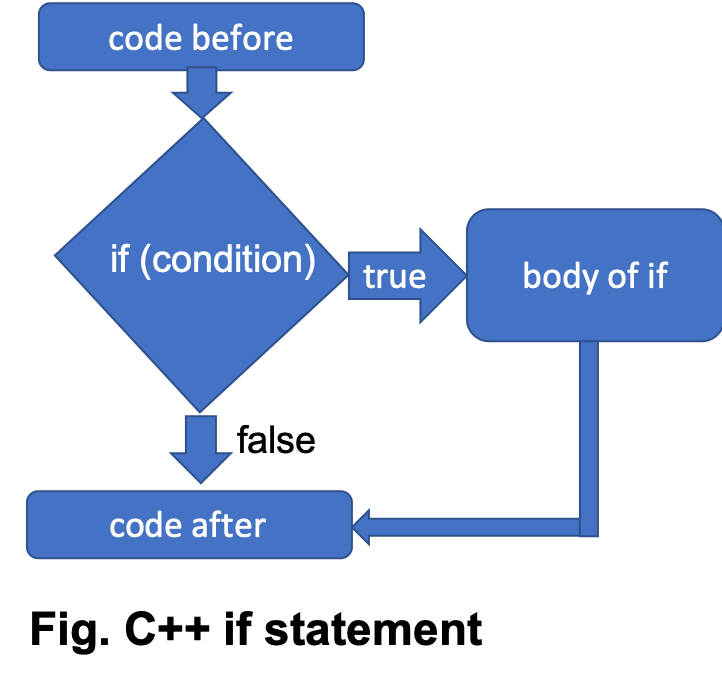
\includegraphics{resources/ifstatement.png}

    \begin{tcolorbox}[breakable, size=fbox, boxrule=1pt, pad at break*=1mm,colback=cellbackground, colframe=cellborder]
\prompt{In}{incolor}{10}{\boxspacing}
\begin{Verbatim}[commandchars=\\\{\}]
\PY{c+c1}{// examples}
\PY{n}{cout} \PY{o}{\PYZlt{}}\PY{o}{\PYZlt{}} \PY{l+s}{\PYZdq{}}\PY{l+s}{stuff before if}\PY{l+s+se}{\PYZbs{}n}\PY{l+s}{\PYZdq{}}\PY{p}{;}
\PY{k}{if} \PY{p}{(}\PY{n+nb}{true}\PY{p}{)} \PY{p}{\PYZob{}} \PY{c+c1}{// true is always true; same as true == true}
    \PY{n}{cout} \PY{o}{\PYZlt{}}\PY{o}{\PYZlt{}} \PY{l+s}{\PYZdq{}}\PY{l+s}{body of if}\PY{l+s+se}{\PYZbs{}n}\PY{l+s}{\PYZdq{}}\PY{p}{;}
\PY{p}{\PYZcb{}}
\PY{n}{cout} \PY{o}{\PYZlt{}}\PY{o}{\PYZlt{}} \PY{l+s}{\PYZdq{}}\PY{l+s}{stuff after if}\PY{l+s+se}{\PYZbs{}n}\PY{l+s}{\PYZdq{}}\PY{p}{;}
\end{Verbatim}
\end{tcolorbox}

    \begin{Verbatim}[commandchars=\\\{\}]
stuff before if
body of if
stuff after if
    \end{Verbatim}

    \begin{tcolorbox}[breakable, size=fbox, boxrule=1pt, pad at break*=1mm,colback=cellbackground, colframe=cellborder]
\prompt{In}{incolor}{11}{\boxspacing}
\begin{Verbatim}[commandchars=\\\{\}]
\PY{n}{cout} \PY{o}{\PYZlt{}}\PY{o}{\PYZlt{}} \PY{l+s}{\PYZdq{}}\PY{l+s}{stuff before if}\PY{l+s+se}{\PYZbs{}n}\PY{l+s}{\PYZdq{}}\PY{p}{;}
\PY{k}{if} \PY{p}{(}\PY{n+nb}{false}\PY{p}{)} \PY{p}{\PYZob{}} \PY{c+c1}{// false always evaluates to false; same as false == true}
    \PY{n}{cout} \PY{o}{\PYZlt{}}\PY{o}{\PYZlt{}} \PY{l+s}{\PYZdq{}}\PY{l+s}{body of if}\PY{l+s+se}{\PYZbs{}n}\PY{l+s}{\PYZdq{}}\PY{p}{;}
\PY{p}{\PYZcb{}}
\PY{n}{cout} \PY{o}{\PYZlt{}}\PY{o}{\PYZlt{}} \PY{l+s}{\PYZdq{}}\PY{l+s}{stuff after if}\PY{l+s+se}{\PYZbs{}n}\PY{l+s}{\PYZdq{}}\PY{p}{;}
\end{Verbatim}
\end{tcolorbox}

    \begin{Verbatim}[commandchars=\\\{\}]
stuff before if
stuff after if
    \end{Verbatim}

    \begin{tcolorbox}[breakable, size=fbox, boxrule=1pt, pad at break*=1mm,colback=cellbackground, colframe=cellborder]
\prompt{In}{incolor}{12}{\boxspacing}
\begin{Verbatim}[commandchars=\\\{\}]
\PY{c+c1}{// check if a given number is positive}
\PY{k+kt}{int} \PY{n}{num}\PY{p}{;}
\end{Verbatim}
\end{tcolorbox}

    \begin{tcolorbox}[breakable, size=fbox, boxrule=1pt, pad at break*=1mm,colback=cellbackground, colframe=cellborder]
\prompt{In}{incolor}{13}{\boxspacing}
\begin{Verbatim}[commandchars=\\\{\}]
\PY{n}{cout} \PY{o}{\PYZlt{}}\PY{o}{\PYZlt{}} \PY{l+s}{\PYZdq{}}\PY{l+s}{enter a whole number: }\PY{l+s}{\PYZdq{}}\PY{p}{;}
\PY{n}{cin} \PY{o}{\PYZgt{}}\PY{o}{\PYZgt{}} \PY{n}{num}\PY{p}{;}
\PY{k}{if} \PY{p}{(}\PY{n}{num} \PY{o}{\PYZgt{}} \PY{l+m+mi}{0}\PY{p}{)} \PY{p}{\PYZob{}}
    \PY{n}{cout} \PY{o}{\PYZlt{}}\PY{o}{\PYZlt{}} \PY{n}{num} \PY{o}{\PYZlt{}}\PY{o}{\PYZlt{}} \PY{l+s}{\PYZdq{}}\PY{l+s}{ is positive}\PY{l+s+se}{\PYZbs{}n}\PY{l+s}{\PYZdq{}}\PY{p}{;}
\PY{p}{\PYZcb{}}
\PY{n}{cout} \PY{o}{\PYZlt{}}\PY{o}{\PYZlt{}} \PY{l+s}{\PYZdq{}}\PY{l+s}{Good bye!}\PY{l+s}{\PYZdq{}}\PY{p}{;}
\end{Verbatim}
\end{tcolorbox}

    \begin{Verbatim}[commandchars=\\\{\}]
enter a whole number: 100
100 is positive
Good bye!
    \end{Verbatim}

    \hypertarget{visualize-one-way-selector-in-pythontutor.com}{%
\subsubsection{\texorpdfstring{Visualize one-way selector in
\href{http://pythontutor.com/cpp.html\#code=\%23include\%20\%3Ciostream\%3E\%0Ausing\%20namespace\%20std\%3B\%0A\%0Aint\%20main\%28\%29\%20\%7B\%0A\%20\%20int\%20num\%20\%3D\%20-9\%3B\%0A\%20\%20if\%20\%28num\%20\%3E\%200\%29\%20\%7B\%0A\%20\%20\%20\%20cout\%20\%3C\%3C\%20num\%20\%3C\%3C\%20\%22\%20is\%20positive\%5Cn\%22\%3B\%0A\%20\%20\%7D\%0A\%20\%20cout\%20\%3C\%3C\%20\%22Good\%20bye!\%22\%3B\%0A\%20\%20return\%200\%3B\%0A\%7D\&curInstr=0\&mode=display\&origin=opt-frontend.js\&py=cpp\&rawInputLstJSON=\%5B\%5D}{pythontutor.com}}{Visualize one-way selector in pythontutor.com}}\label{visualize-one-way-selector-in-pythontutor.com}}

\hypertarget{two-way-selector}{%
\subsubsection{Two-way selector}\label{two-way-selector}}

\begin{itemize}
\tightlist
\item
  provides alternative execution
\item
  analogy is a true/false type question

  \begin{itemize}
  \tightlist
  \item
    you have to pick one or the other
  \end{itemize}
\item
  syntax:
\end{itemize}

\begin{Shaded}
\begin{Highlighting}[]
    \ControlFlowTok{if} \OperatorTok{(}\NormalTok{condition}\OperatorTok{)} \OperatorTok{\{}
        \CommentTok{// body of if}
    \OperatorTok{\}}
    \ControlFlowTok{else} \OperatorTok{\{}
        \CommentTok{// otherwise, body of else}
    \OperatorTok{\}}
\end{Highlighting}
\end{Shaded}

\begin{itemize}
\tightlist
\item
  if the condition is true, body of if executes
\item
  oterwise, body of else executes
\item
  the following flowchart demonstrates the flow of if else statement
\end{itemize}

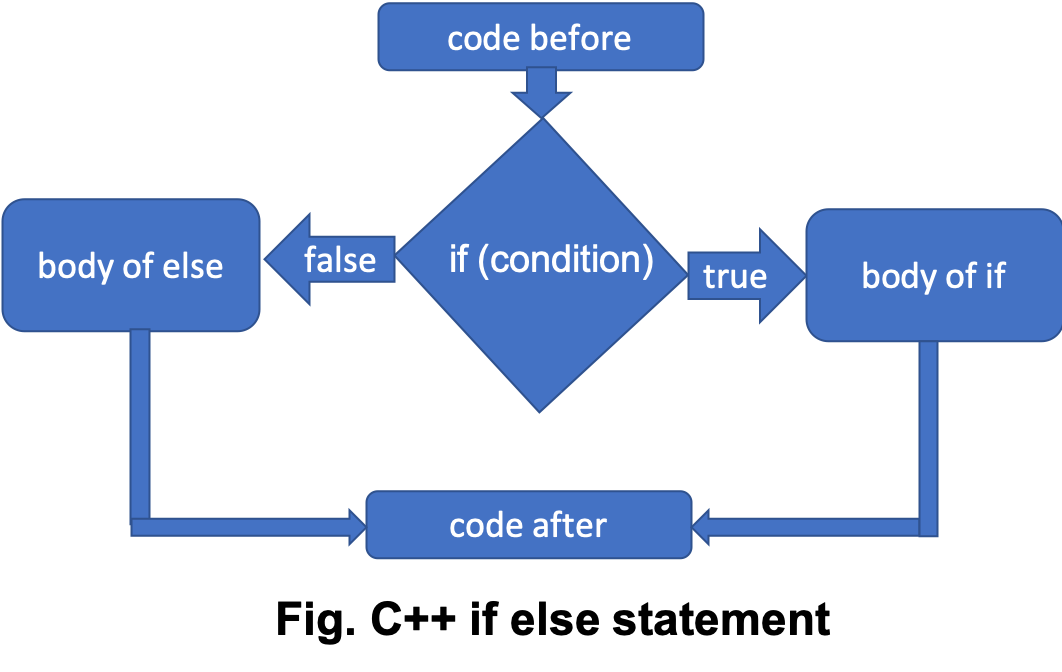
\includegraphics{resources/ifelsestatement.png}

    \begin{tcolorbox}[breakable, size=fbox, boxrule=1pt, pad at break*=1mm,colback=cellbackground, colframe=cellborder]
\prompt{In}{incolor}{14}{\boxspacing}
\begin{Verbatim}[commandchars=\\\{\}]
\PY{c+c1}{// determine if the given number is positive or negative}
\PY{n}{cout} \PY{o}{\PYZlt{}}\PY{o}{\PYZlt{}} \PY{l+s}{\PYZdq{}}\PY{l+s}{Enter a whole number: }\PY{l+s}{\PYZdq{}}\PY{p}{;}
\PY{n}{cin} \PY{o}{\PYZgt{}}\PY{o}{\PYZgt{}} \PY{n}{num}\PY{p}{;}
\PY{k}{if} \PY{p}{(}\PY{n}{num} \PY{o}{\PYZgt{}} \PY{l+m+mi}{0}\PY{p}{)} \PY{p}{\PYZob{}}
    \PY{n}{cout} \PY{o}{\PYZlt{}}\PY{o}{\PYZlt{}} \PY{n}{num} \PY{o}{\PYZlt{}}\PY{o}{\PYZlt{}} \PY{l+s}{\PYZdq{}}\PY{l+s}{ is positive}\PY{l+s+se}{\PYZbs{}n}\PY{l+s}{\PYZdq{}}\PY{p}{;}
\PY{p}{\PYZcb{}}
\PY{k}{else} \PY{p}{\PYZob{}}
    \PY{n}{cout} \PY{o}{\PYZlt{}}\PY{o}{\PYZlt{}} \PY{n}{num} \PY{o}{\PYZlt{}}\PY{o}{\PYZlt{}} \PY{l+s}{\PYZdq{}}\PY{l+s}{ is negative}\PY{l+s+se}{\PYZbs{}n}\PY{l+s}{\PYZdq{}}\PY{p}{;}
\PY{p}{\PYZcb{}}
\PY{n}{cout} \PY{o}{\PYZlt{}}\PY{o}{\PYZlt{}} \PY{l+s}{\PYZdq{}}\PY{l+s}{Good bye!}\PY{l+s}{\PYZdq{}}\PY{p}{;}
\PY{c+c1}{// run it few times providing +ve and \PYZhy{}ve numbers}
\end{Verbatim}
\end{tcolorbox}

    \begin{Verbatim}[commandchars=\\\{\}]
Enter a whole number: 99
99 is positive
Good bye!
    \end{Verbatim}

            \begin{tcolorbox}[breakable, size=fbox, boxrule=.5pt, pad at break*=1mm, opacityfill=0]
\prompt{Out}{outcolor}{14}{\boxspacing}
\begin{Verbatim}[commandchars=\\\{\}]
@0x10c49bed0
\end{Verbatim}
\end{tcolorbox}
        
    \hypertarget{visualize-two-way-selector-in-pythontutor.com}{%
\subsubsection{\texorpdfstring{Visualize two-way selector in
\href{http://pythontutor.com/cpp.html\#code=\%23include\%20\%3Ciostream\%3E\%0Ausing\%20namespace\%20std\%3B\%0A\%0Aint\%20main\%28\%29\%20\%7B\%0A\%20\%20int\%20num1\%20\%3D\%20100\%3B\%0A\%20\%20int\%20num2\%20\%3D\%20200\%3B\%0A\%20\%20if\%20\%28num1\%20\%3E\%3D\%20num2\%29\%0A\%20\%20\%20\%20cout\%20\%3C\%3C\%20num1\%20\%3C\%3C\%20\%22\%20is\%20greater\%20than\%20or\%20equal\%20to\%20\%22\%20\%3C\%3C\%20num2\%20\%3C\%3C\%20endl\%3B\%0A\%20\%20else\%0A\%20\%20\%20\%20cout\%20\%3C\%3C\%20num2\%20\%3C\%3C\%20\%22\%20is\%20greater\%20than\%20\%22\%20\%3C\%3C\%20num1\%20\%3C\%3C\%20endl\%3B\%0A\%20\%20\%20\%20\%0A\%20\%20cout\%20\%3C\%3C\%20\%22Good\%20Bye!\%22\%3B\%0A\%20\%20return\%200\%3B\%0A\%7D\&curInstr=0\&mode=display\&origin=opt-frontend.js\&py=cpp\&rawInputLstJSON=\%5B\%5D}{pythontutor.com}}{Visualize two-way selector in pythontutor.com}}\label{visualize-two-way-selector-in-pythontutor.com}}

\hypertarget{multi-way-selector}{%
\subsubsection{Multi-way selector}\label{multi-way-selector}}

\begin{itemize}
\tightlist
\item
  sometimes one may have to pick one outcome from several options

  \begin{itemize}
  \tightlist
  \item
    analogy is multiple-choice question with only one correct answer!
  \end{itemize}
\item
  we can achieve this by chaining a series of \texttt{else\ if}s
\item
  also called chained conditionals
\item
  syntax:
\end{itemize}

\begin{Shaded}
\begin{Highlighting}[]
    \ControlFlowTok{if} \OperatorTok{(}\NormalTok{condition}\OperatorTok{)} \OperatorTok{\{}
        \CommentTok{// first if block}
    \OperatorTok{\}}
    \ControlFlowTok{else} \ControlFlowTok{if}\OperatorTok{(}\NormalTok{condition}\OperatorTok{)} \OperatorTok{\{}
        \CommentTok{// 2nd if block}
    \OperatorTok{\}}
    \ControlFlowTok{else} \ControlFlowTok{if}\OperatorTok{(}\NormalTok{condition}\OperatorTok{)} \OperatorTok{\{}
        \CommentTok{// 3rd if block}
    \OperatorTok{\}}
    \OperatorTok{...}
    \ControlFlowTok{else} \OperatorTok{\{}
        \CommentTok{// alternative}
    \OperatorTok{\}}
\end{Highlighting}
\end{Shaded}

\begin{itemize}
\tightlist
\item
  check condition starting from the first \textbf{if statement}
\item
  if the condition is true, execute the corresponding if block

  \begin{itemize}
  \tightlist
  \item
    skip the rest of the chained conditions if any
  \end{itemize}
\item
  otherwise, check next condition

  \begin{itemize}
  \tightlist
  \item
    so on and so forth\ldots{}
  \end{itemize}
\item
  execute else alternative if not a single condition is evaluated true
\item
  the following flowchart depicts the chained conditional execution
\end{itemize}

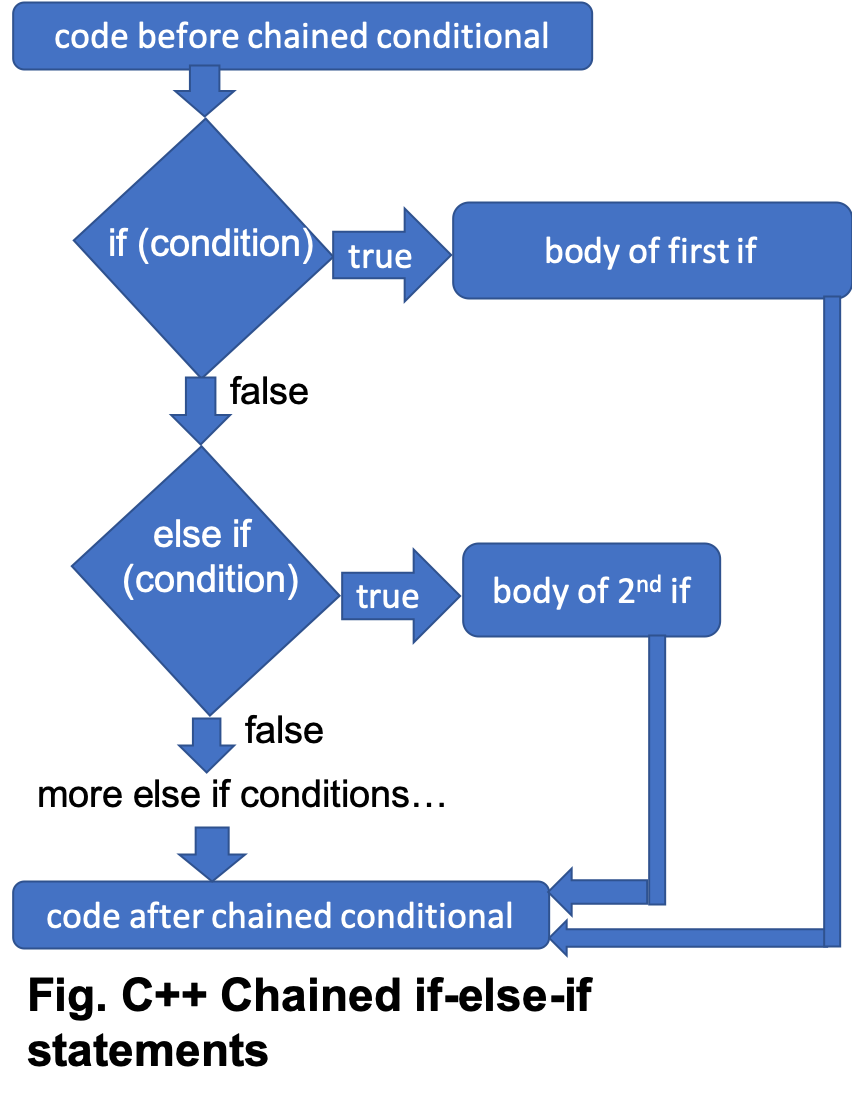
\includegraphics{resources/multi-wayselector.png}

\hypertarget{note}{%
\subsubsection{NOTE:}\label{note}}

\begin{itemize}
\tightlist
\item
  since the condition is checked from top to bottom, the order of
  checking condition matters in some problems!
\end{itemize}

    \begin{tcolorbox}[breakable, size=fbox, boxrule=1pt, pad at break*=1mm,colback=cellbackground, colframe=cellborder]
\prompt{In}{incolor}{15}{\boxspacing}
\begin{Verbatim}[commandchars=\\\{\}]
\PY{c+c1}{// determine if a given number is 0, positive, or negative}
\PY{n}{cout} \PY{o}{\PYZlt{}}\PY{o}{\PYZlt{}} \PY{l+s}{\PYZdq{}}\PY{l+s}{enter a whole number: }\PY{l+s}{\PYZdq{}}\PY{p}{;}
\PY{n}{cin} \PY{o}{\PYZgt{}}\PY{o}{\PYZgt{}} \PY{n}{num}\PY{p}{;}
\PY{k}{if} \PY{p}{(}\PY{n}{num} \PY{o}{\PYZgt{}} \PY{l+m+mi}{0}\PY{p}{)}
    \PY{c+c1}{// if a block has only one statment; \PYZob{}\PYZcb{} can be ignored!}
    \PY{n}{cout} \PY{o}{\PYZlt{}}\PY{o}{\PYZlt{}} \PY{n}{num} \PY{o}{\PYZlt{}}\PY{o}{\PYZlt{}} \PY{l+s}{\PYZdq{}}\PY{l+s}{ is positive}\PY{l+s+se}{\PYZbs{}n}\PY{l+s}{\PYZdq{}}\PY{p}{;}
\PY{k}{else} \PY{k}{if} \PY{p}{(}\PY{n}{num} \PY{o}{\PYZlt{}} \PY{l+m+mi}{0}\PY{p}{)}
    \PY{n}{cout} \PY{o}{\PYZlt{}}\PY{o}{\PYZlt{}} \PY{n}{num} \PY{o}{\PYZlt{}}\PY{o}{\PYZlt{}} \PY{l+s}{\PYZdq{}}\PY{l+s}{ is negative}\PY{l+s+se}{\PYZbs{}n}\PY{l+s}{\PYZdq{}}\PY{p}{;}
\PY{k}{else}
    \PY{n}{cout} \PY{o}{\PYZlt{}}\PY{o}{\PYZlt{}} \PY{l+s}{\PYZdq{}}\PY{l+s}{the entered number is 0}\PY{l+s+se}{\PYZbs{}n}\PY{l+s}{\PYZdq{}}\PY{p}{;}

\PY{n}{cout} \PY{o}{\PYZlt{}}\PY{o}{\PYZlt{}} \PY{l+s}{\PYZdq{}}\PY{l+s}{Good bye!}\PY{l+s}{\PYZdq{}}\PY{p}{;}
\end{Verbatim}
\end{tcolorbox}

    \begin{Verbatim}[commandchars=\\\{\}]
enter a whole number: -9
-9 is negative
Good bye!
    \end{Verbatim}

    \hypertarget{demo-program-that-determines-letter-grade-a-f-given-numeric-grade-0-100}{%
\subsubsection{Demo program that determines letter grade (A-F) given
numeric grade
(0-100)}\label{demo-program-that-determines-letter-grade-a-f-given-numeric-grade-0-100}}

\begin{itemize}
\tightlist
\item
  write a program that converts numeric grade into the corresponding
  letter grade
\item
  letter grade criteria:
\end{itemize}

\begin{verbatim}
    grade >= 90 -> A
    grade >= 80 -> B
    grade >= 70 -> C
    grade >= 60 -> D
    grade < 60  -> F
\end{verbatim}

    \begin{tcolorbox}[breakable, size=fbox, boxrule=1pt, pad at break*=1mm,colback=cellbackground, colframe=cellborder]
\prompt{In}{incolor}{16}{\boxspacing}
\begin{Verbatim}[commandchars=\\\{\}]
\PY{c+c1}{// variable to store the numeric grade}
\PY{k+kt}{float} \PY{n}{grade}\PY{p}{;}
\end{Verbatim}
\end{tcolorbox}

    \begin{tcolorbox}[breakable, size=fbox, boxrule=1pt, pad at break*=1mm,colback=cellbackground, colframe=cellborder]
\prompt{In}{incolor}{17}{\boxspacing}
\begin{Verbatim}[commandchars=\\\{\}]
\PY{c+c1}{// Implementation I}
\PY{c+c1}{// does this solution give correct answer?}
\PY{c+c1}{// order of checking condition matters!}
\PY{n}{cout} \PY{o}{\PYZlt{}}\PY{o}{\PYZlt{}} \PY{l+s}{\PYZdq{}}\PY{l+s}{Enter a grade: }\PY{l+s}{\PYZdq{}}\PY{p}{;}
\PY{n}{cin} \PY{o}{\PYZgt{}}\PY{o}{\PYZgt{}} \PY{n}{grade}\PY{p}{;}

\PY{k}{if} \PY{p}{(}\PY{n}{grade} \PY{o}{\PYZlt{}} \PY{l+m+mi}{60}\PY{p}{)}
    \PY{n}{cout} \PY{o}{\PYZlt{}}\PY{o}{\PYZlt{}} \PY{n}{grade} \PY{o}{\PYZlt{}}\PY{o}{\PYZlt{}} \PY{l+s}{\PYZdq{}}\PY{l+s}{is an F!}\PY{l+s+se}{\PYZbs{}n}\PY{l+s}{\PYZdq{}}\PY{p}{;}
\PY{k}{else} \PY{k}{if}\PY{p}{(}\PY{n}{grade} \PY{o}{\PYZgt{}}\PY{o}{=} \PY{l+m+mi}{60}\PY{p}{)}
    \PY{n}{cout} \PY{o}{\PYZlt{}}\PY{o}{\PYZlt{}} \PY{n}{grade} \PY{o}{\PYZlt{}}\PY{o}{\PYZlt{}} \PY{l+s}{\PYZdq{}}\PY{l+s}{ is a D.}\PY{l+s+se}{\PYZbs{}n}\PY{l+s}{\PYZdq{}}\PY{p}{;}
\PY{k}{else} \PY{k}{if}\PY{p}{(}\PY{n}{grade} \PY{o}{\PYZgt{}}\PY{o}{=} \PY{l+m+mi}{70}\PY{p}{)}
    \PY{n}{cout} \PY{o}{\PYZlt{}}\PY{o}{\PYZlt{}} \PY{n}{grade} \PY{o}{\PYZlt{}}\PY{o}{\PYZlt{}} \PY{l+s}{\PYZdq{}}\PY{l+s}{is a C.}\PY{l+s+se}{\PYZbs{}n}\PY{l+s}{\PYZdq{}}\PY{p}{;}
\PY{k}{else} \PY{k}{if} \PY{p}{(}\PY{n}{grade} \PY{o}{\PYZgt{}}\PY{o}{=} \PY{l+m+mi}{80}\PY{p}{)}
    \PY{n}{cout} \PY{o}{\PYZlt{}}\PY{o}{\PYZlt{}} \PY{n}{grade} \PY{o}{\PYZlt{}}\PY{o}{\PYZlt{}} \PY{l+s}{\PYZdq{}}\PY{l+s}{ is a B.}\PY{l+s+se}{\PYZbs{}n}\PY{l+s}{\PYZdq{}}\PY{p}{;}
\PY{k}{else} \PY{k}{if} \PY{p}{(}\PY{n}{grade} \PY{o}{\PYZgt{}}\PY{o}{=} \PY{l+m+mi}{90}\PY{p}{)}
    \PY{n}{cout} \PY{o}{\PYZlt{}}\PY{o}{\PYZlt{}} \PY{n}{grade} \PY{o}{\PYZlt{}}\PY{o}{\PYZlt{}} \PY{l+s}{\PYZdq{}}\PY{l+s}{ is an A!}\PY{l+s+se}{\PYZbs{}n}\PY{l+s}{\PYZdq{}}\PY{p}{;}

\PY{n}{cout} \PY{o}{\PYZlt{}}\PY{o}{\PYZlt{}} \PY{l+s}{\PYZdq{}}\PY{l+s}{Good bye!}\PY{l+s}{\PYZdq{}}\PY{p}{;}
\end{Verbatim}
\end{tcolorbox}

    \begin{Verbatim}[commandchars=\\\{\}]
Enter a grade: 90
90 is a D.
Good bye!
    \end{Verbatim}

    \begin{tcolorbox}[breakable, size=fbox, boxrule=1pt, pad at break*=1mm,colback=cellbackground, colframe=cellborder]
\prompt{In}{incolor}{18}{\boxspacing}
\begin{Verbatim}[commandchars=\\\{\}]
\PY{c+c1}{// Implementation II}
\PY{c+c1}{// how about this solution; does this give correct answer?}
\PY{n}{cout} \PY{o}{\PYZlt{}}\PY{o}{\PYZlt{}} \PY{l+s}{\PYZdq{}}\PY{l+s}{Enter a grade: }\PY{l+s}{\PYZdq{}}\PY{p}{;}
\PY{n}{cin} \PY{o}{\PYZgt{}}\PY{o}{\PYZgt{}} \PY{n}{grade}\PY{p}{;}

\PY{k}{if} \PY{p}{(}\PY{n}{grade} \PY{o}{\PYZgt{}}\PY{o}{=} \PY{l+m+mi}{90}\PY{p}{)} \PY{p}{\PYZob{}}
    \PY{n}{cout} \PY{o}{\PYZlt{}}\PY{o}{\PYZlt{}} \PY{n}{grade} \PY{o}{\PYZlt{}}\PY{o}{\PYZlt{}} \PY{l+s}{\PYZdq{}}\PY{l+s}{ is an A! :))}\PY{l+s+se}{\PYZbs{}n}\PY{l+s}{\PYZdq{}}\PY{p}{;}
    \PY{n}{cout} \PY{o}{\PYZlt{}}\PY{o}{\PYZlt{}} \PY{l+s}{\PYZdq{}}\PY{l+s}{Awesome job!}\PY{l+s+se}{\PYZbs{}n}\PY{l+s}{\PYZdq{}}\PY{p}{;}
\PY{p}{\PYZcb{}}
\PY{k}{else} \PY{k}{if}\PY{p}{(}\PY{n}{grade} \PY{o}{\PYZgt{}}\PY{o}{=} \PY{l+m+mi}{80}\PY{p}{)} \PY{p}{\PYZob{}}
    \PY{n}{cout} \PY{o}{\PYZlt{}}\PY{o}{\PYZlt{}} \PY{n}{grade} \PY{o}{\PYZlt{}}\PY{o}{\PYZlt{}} \PY{l+s}{\PYZdq{}}\PY{l+s}{ is a B. :)}\PY{l+s+se}{\PYZbs{}n}\PY{l+s}{\PYZdq{}}\PY{p}{;}
    \PY{n}{cout} \PY{o}{\PYZlt{}}\PY{o}{\PYZlt{}} \PY{l+s}{\PYZdq{}}\PY{l+s}{Great job! So close to acing... keep working!}\PY{l+s+se}{\PYZbs{}n}\PY{l+s}{\PYZdq{}}\PY{p}{;}
\PY{p}{\PYZcb{}}
\PY{k}{else} \PY{k}{if}\PY{p}{(}\PY{n}{grade} \PY{o}{\PYZgt{}}\PY{o}{=} \PY{l+m+mi}{70}\PY{p}{)} \PY{p}{\PYZob{}}
    \PY{n}{cout} \PY{o}{\PYZlt{}}\PY{o}{\PYZlt{}} \PY{n}{grade} \PY{o}{\PYZlt{}}\PY{o}{\PYZlt{}} \PY{l+s}{\PYZdq{}}\PY{l+s}{ is a C. :|}\PY{l+s+se}{\PYZbs{}n}\PY{l+s}{\PYZdq{}}\PY{p}{;}
    \PY{n}{cout} \PY{o}{\PYZlt{}}\PY{o}{\PYZlt{}} \PY{l+s}{\PYZdq{}}\PY{l+s}{Good job! work harder to get a B or an A}\PY{l+s+se}{\PYZbs{}n}\PY{l+s}{\PYZdq{}}\PY{p}{;}
\PY{p}{\PYZcb{}}
\PY{k}{else} \PY{k}{if}\PY{p}{(}\PY{n}{grade} \PY{o}{\PYZgt{}}\PY{o}{=} \PY{l+m+mi}{60}\PY{p}{)} \PY{p}{\PYZob{}}
    \PY{n}{cout} \PY{o}{\PYZlt{}}\PY{o}{\PYZlt{}} \PY{n}{grade} \PY{o}{\PYZlt{}}\PY{o}{\PYZlt{}} \PY{l+s}{\PYZdq{}}\PY{l+s}{ is a D. :(}\PY{l+s+se}{\PYZbs{}n}\PY{l+s}{\PYZdq{}}\PY{p}{;}
    \PY{n}{cout} \PY{o}{\PYZlt{}}\PY{o}{\PYZlt{}} \PY{l+s}{\PYZdq{}}\PY{l+s}{Sorry, D isn\PYZsq{}t good enought to move on to CS2}\PY{l+s+se}{\PYZbs{}n}\PY{l+s}{. Work very hard!}\PY{l+s}{\PYZdq{}}\PY{p}{;}
\PY{p}{\PYZcb{}}
\PY{k}{else} \PY{p}{\PYZob{}}
    \PY{n}{cout} \PY{o}{\PYZlt{}}\PY{o}{\PYZlt{}} \PY{n}{grade} \PY{o}{\PYZlt{}}\PY{o}{\PYZlt{}} \PY{l+s}{\PYZdq{}}\PY{l+s}{ is an F. :((}\PY{l+s+se}{\PYZbs{}n}\PY{l+s}{\PYZdq{}}\PY{p}{;}
    \PY{n}{cout} \PY{o}{\PYZlt{}}\PY{o}{\PYZlt{}} \PY{l+s}{\PYZdq{}}\PY{l+s}{Sorry, that\PYZsq{}s a fail. Work really really hard to pass!!}\PY{l+s+se}{\PYZbs{}n}\PY{l+s}{\PYZdq{}}\PY{p}{;}
\PY{p}{\PYZcb{}}

\PY{n}{cout} \PY{o}{\PYZlt{}}\PY{o}{\PYZlt{}} \PY{l+s}{\PYZdq{}}\PY{l+s}{Good bye!}\PY{l+s+se}{\PYZbs{}n}\PY{l+s}{\PYZdq{}}\PY{p}{;}
\end{Verbatim}
\end{tcolorbox}

    \begin{Verbatim}[commandchars=\\\{\}]
Enter a grade: 90
90 is an A! :))
Awesome job!
Good bye!
    \end{Verbatim}

    \begin{tcolorbox}[breakable, size=fbox, boxrule=1pt, pad at break*=1mm,colback=cellbackground, colframe=cellborder]
\prompt{In}{incolor}{19}{\boxspacing}
\begin{Verbatim}[commandchars=\\\{\}]
\PY{c+c1}{// Implementation III \PYZhy{} using function}
\PY{k+kt}{char} \PY{n+nf}{find\PYZus{}letter\PYZus{}grade}\PY{p}{(}\PY{k+kt}{float} \PY{n}{grade}\PY{p}{)} \PY{p}{\PYZob{}}
    \PY{k}{if} \PY{p}{(}\PY{n}{grade} \PY{o}{\PYZgt{}}\PY{o}{=} \PY{l+m+mi}{90}\PY{p}{)}
        \PY{k}{return} \PY{l+s+sc}{\PYZsq{}}\PY{l+s+sc}{A}\PY{l+s+sc}{\PYZsq{}}\PY{p}{;}
    \PY{k}{else} \PY{k}{if}\PY{p}{(}\PY{n}{grade} \PY{o}{\PYZgt{}}\PY{o}{=} \PY{l+m+mi}{80}\PY{p}{)}
        \PY{k}{return} \PY{l+s+sc}{\PYZsq{}}\PY{l+s+sc}{B}\PY{l+s+sc}{\PYZsq{}}\PY{p}{;}
    \PY{k}{else} \PY{k}{if}\PY{p}{(}\PY{n}{grade} \PY{o}{\PYZgt{}}\PY{o}{=} \PY{l+m+mi}{70}\PY{p}{)}
        \PY{k}{return} \PY{l+s+sc}{\PYZsq{}}\PY{l+s+sc}{C}\PY{l+s+sc}{\PYZsq{}}\PY{p}{;}
    \PY{k}{else} \PY{k}{if}\PY{p}{(}\PY{n}{grade} \PY{o}{\PYZgt{}}\PY{o}{=} \PY{l+m+mi}{60}\PY{p}{)}
        \PY{k}{return} \PY{l+s+sc}{\PYZsq{}}\PY{l+s+sc}{D}\PY{l+s+sc}{\PYZsq{}}\PY{p}{;}
    \PY{k}{else}
        \PY{k}{return} \PY{l+s+sc}{\PYZsq{}}\PY{l+s+sc}{F}\PY{l+s+sc}{\PYZsq{}}\PY{p}{;}
\PY{p}{\PYZcb{}}
\end{Verbatim}
\end{tcolorbox}

    \begin{tcolorbox}[breakable, size=fbox, boxrule=1pt, pad at break*=1mm,colback=cellbackground, colframe=cellborder]
\prompt{In}{incolor}{20}{\boxspacing}
\begin{Verbatim}[commandchars=\\\{\}]
\PY{c+c1}{// manually test find\PYZus{}letter\PYZus{}grade function}
\PY{n}{cout} \PY{o}{\PYZlt{}}\PY{o}{\PYZlt{}} \PY{l+s}{\PYZdq{}}\PY{l+s}{Enter a numeric grade: }\PY{l+s}{\PYZdq{}}\PY{p}{;}
\PY{n}{cin} \PY{o}{\PYZgt{}}\PY{o}{\PYZgt{}} \PY{n}{grade}\PY{p}{;}
\PY{k+kt}{char} \PY{n}{l\PYZus{}grade} \PY{o}{=} \PY{n}{find\PYZus{}letter\PYZus{}grade}\PY{p}{(}\PY{n}{grade}\PY{p}{)}\PY{p}{;}
\PY{n}{cout} \PY{o}{\PYZlt{}}\PY{o}{\PYZlt{}} \PY{n}{grade} \PY{o}{\PYZlt{}}\PY{o}{\PYZlt{}} \PY{l+s}{\PYZdq{}}\PY{l+s}{ is equivalent to }\PY{l+s}{\PYZdq{}} \PY{o}{\PYZlt{}}\PY{o}{\PYZlt{}} \PY{n}{l\PYZus{}grade} \PY{o}{\PYZlt{}}\PY{o}{\PYZlt{}} \PY{n}{endl}\PY{p}{;}
\PY{k}{if} \PY{p}{(}\PY{n}{l\PYZus{}grade} \PY{o}{=}\PY{o}{=} \PY{l+s+sc}{\PYZsq{}}\PY{l+s+sc}{A}\PY{l+s+sc}{\PYZsq{}}\PY{p}{)}
    \PY{n}{cout} \PY{o}{\PYZlt{}}\PY{o}{\PYZlt{}} \PY{l+s}{\PYZdq{}}\PY{l+s}{Awesome job! :))}\PY{l+s+se}{\PYZbs{}n}\PY{l+s}{\PYZdq{}}\PY{p}{;}
\end{Verbatim}
\end{tcolorbox}

    \begin{Verbatim}[commandchars=\\\{\}]
Enter a numeric grade: 75
75 is equivalent to C
    \end{Verbatim}

    \begin{tcolorbox}[breakable, size=fbox, boxrule=1pt, pad at break*=1mm,colback=cellbackground, colframe=cellborder]
\prompt{In}{incolor}{21}{\boxspacing}
\begin{Verbatim}[commandchars=\\\{\}]
\PY{c+c1}{// automatically test find\PYZus{}letter\PYZus{}grade function}
\PY{k+kt}{void} \PY{n+nf}{test\PYZus{}find\PYZus{}letter\PYZus{}grade}\PY{p}{(}\PY{p}{)} \PY{p}{\PYZob{}}
    \PY{n}{assert}\PY{p}{(}\PY{n}{find\PYZus{}letter\PYZus{}grade}\PY{p}{(}\PY{l+m+mi}{100}\PY{p}{)} \PY{o}{=}\PY{o}{=} \PY{l+s+sc}{\PYZsq{}}\PY{l+s+sc}{A}\PY{l+s+sc}{\PYZsq{}}\PY{p}{)}\PY{p}{;}
    \PY{n}{assert}\PY{p}{(}\PY{n}{find\PYZus{}letter\PYZus{}grade}\PY{p}{(}\PY{l+m+mi}{40}\PY{p}{)} \PY{o}{=}\PY{o}{=} \PY{l+s+sc}{\PYZsq{}}\PY{l+s+sc}{F}\PY{l+s+sc}{\PYZsq{}}\PY{p}{)}\PY{p}{;}
    \PY{n}{assert}\PY{p}{(}\PY{n}{find\PYZus{}letter\PYZus{}grade}\PY{p}{(}\PY{l+m+mi}{89}\PY{p}{)} \PY{o}{=}\PY{o}{=} \PY{l+s+sc}{\PYZsq{}}\PY{l+s+sc}{B}\PY{l+s+sc}{\PYZsq{}}\PY{p}{)}\PY{p}{;}
    \PY{c+c1}{// TODO: test for every possible outcome}
    \PY{n}{cerr} \PY{o}{\PYZlt{}}\PY{o}{\PYZlt{}} \PY{l+s}{\PYZdq{}}\PY{l+s}{all test casses passed!}\PY{l+s}{\PYZdq{}} \PY{o}{\PYZlt{}}\PY{o}{\PYZlt{}} \PY{n}{endl}\PY{p}{;}
\PY{p}{\PYZcb{}}
\end{Verbatim}
\end{tcolorbox}

    \begin{tcolorbox}[breakable, size=fbox, boxrule=1pt, pad at break*=1mm,colback=cellbackground, colframe=cellborder]
\prompt{In}{incolor}{22}{\boxspacing}
\begin{Verbatim}[commandchars=\\\{\}]
\PY{n}{test\PYZus{}find\PYZus{}letter\PYZus{}grade}\PY{p}{(}\PY{p}{)}\PY{p}{;}
\end{Verbatim}
\end{tcolorbox}

    \begin{Verbatim}[commandchars=\\\{\}]
all test casses passed!
    \end{Verbatim}

    \hypertarget{visualize-multi-way-selector-in-pythontutor.com}{%
\subsubsection{\texorpdfstring{Visualize multi-way selector in
\href{http://pythontutor.com/cpp.html\#code=//\%20program\%20to\%20determine\%20day\%20of\%20the\%20week\%20given\%20number\%0A//\%201-7\%20\%28sunday\%20to\%20saturday\%29\%0A\%23include\%20\%3Ciostream\%3E\%0Ausing\%20namespace\%20std\%3B\%0A\%0Aint\%20main\%28\%29\%20\%7B\%0A\%20\%20int\%20day\%20\%3D\%200\%3B\%0A\%20\%20if\%20\%28day\%20\%3D\%3D\%201\%29\%0A\%20\%20\%20\%20cout\%20\%3C\%3C\%20day\%20\%3C\%3C\%20\%22\%20is\%20Sunday\%5Cn\%22\%3B\%0A\%20\%20else\%20if\%20\%28day\%20\%3D\%3D\%202\%29\%0A\%20\%20\%20\%20cout\%20\%3C\%3C\%20day\%20\%3C\%3C\%20\%22\%20is\%20Monday\%5Cn\%22\%3B\%0A\%20\%20else\%20if\%20\%28day\%20\%3D\%3D\%203\%29\%0A\%20\%20\%20\%20cout\%20\%3C\%3C\%20day\%20\%3C\%3C\%20\%22\%20is\%20Tuesday\%5Cn\%22\%3B\%0A\%20\%20else\%20if\%20\%28day\%20\%3D\%3D\%204\%29\%0A\%20\%20\%20\%20cout\%20\%3C\%3C\%20day\%20\%3C\%3C\%20\%22\%20is\%20Wednesday\%5Cn\%22\%3B\%0A\%20\%20else\%20if\%20\%28day\%20\%3D\%3D\%205\%29\%0A\%20\%20\%20\%20cout\%20\%3C\%3C\%20day\%20\%3C\%3C\%20\%22\%20is\%20Thursday\%5Cn\%22\%3B\%0A\%20\%20else\%20if\%20\%28day\%20\%3D\%3D\%206\%29\%0A\%20\%20\%20\%20cout\%20\%3C\%3C\%20day\%20\%3C\%3C\%20\%22\%20is\%20Friday\%5Cn\%22\%3B\%0A\%20\%20else\%20if\%20\%28day\%20\%3D\%3D\%207\%29\%0A\%20\%20\%20\%20cout\%20\%3C\%3C\%20day\%20\%3C\%3C\%20\%22\%20is\%20Saturday\%5Cn\%22\%3B\%0A\%20\%20else\%0A\%20\%20\%20\%20cout\%20\%3C\%3C\%20day\%20\%3C\%3C\%20\%22\%20is\%20not\%20a\%20valid\%20day!\%22\%3B\%0A\%20\%20\%20\%20\%0A\%20\%20cout\%20\%3C\%3C\%20\%22Good\%20bye...\%5Cn\%22\%3B\%0A\%20\%20return\%200\%3B\%0A\%7D\&curInstr=0\&mode=display\&origin=opt-frontend.js\&py=cpp\&rawInputLstJSON=\%5B\%5D}{pythontutor.com}}{Visualize multi-way selector in pythontutor.com}}\label{visualize-multi-way-selector-in-pythontutor.com}}

    \hypertarget{nested-conditionals}{%
\subsection{Nested conditionals}\label{nested-conditionals}}

\begin{itemize}
\tightlist
\item
  one or more type of conditional statements can be nested inside
  another conditional statement
\item
  syntax:
\end{itemize}

\begin{Shaded}
\begin{Highlighting}[]
    \ControlFlowTok{if} \OperatorTok{(}\NormalTok{condition}\OperatorTok{)} \OperatorTok{\{}
        \CommentTok{// do something}
        \ControlFlowTok{if} \OperatorTok{(}\NormalTok{condition}\OperatorTok{)} \OperatorTok{\{}
            \CommentTok{// do something..}
        \OperatorTok{\}}

        \ControlFlowTok{if} \OperatorTok{(}\NormalTok{condition}\OperatorTok{)} \OperatorTok{\{}
            \CommentTok{// do something}
        \OperatorTok{\}}
        \ControlFlowTok{else} \OperatorTok{\{}
            \CommentTok{// do something else}
        \OperatorTok{\}}

    \OperatorTok{\}}
    \ControlFlowTok{else} \OperatorTok{\{}
        \CommentTok{// do something else...}
        \ControlFlowTok{if} \OperatorTok{(}\NormalTok{condition}\OperatorTok{)} \OperatorTok{\{}
            \CommentTok{// do something}
        \OperatorTok{\}}
    \OperatorTok{\}}
\end{Highlighting}
\end{Shaded}

    \begin{tcolorbox}[breakable, size=fbox, boxrule=1pt, pad at break*=1mm,colback=cellbackground, colframe=cellborder]
\prompt{In}{incolor}{24}{\boxspacing}
\begin{Verbatim}[commandchars=\\\{\}]
\PY{c+c1}{// a program that determines if a given number is 0, even or odd and positive or negative}
\PY{c+c1}{// the order of condition doesn\PYZsq{}t matter in this example}
\PY{n}{cout} \PY{o}{\PYZlt{}}\PY{o}{\PYZlt{}} \PY{l+s}{\PYZdq{}}\PY{l+s}{enter a whole number: }\PY{l+s}{\PYZdq{}}\PY{p}{;}
\PY{n}{cin} \PY{o}{\PYZgt{}}\PY{o}{\PYZgt{}} \PY{n}{num}\PY{p}{;}
\PY{k}{if} \PY{p}{(}\PY{n}{num} \PY{o}{\PYZgt{}} \PY{l+m+mi}{0}\PY{p}{)} \PY{p}{\PYZob{}}
    \PY{n}{cout} \PY{o}{\PYZlt{}}\PY{o}{\PYZlt{}} \PY{n}{num} \PY{o}{\PYZlt{}}\PY{o}{\PYZlt{}} \PY{l+s}{\PYZdq{}}\PY{l+s}{ is positive }\PY{l+s}{\PYZdq{}}\PY{p}{;}
    \PY{c+c1}{// check if the number is even or odd}
    \PY{k}{if} \PY{p}{(}\PY{n}{num} \PY{o}{\PYZpc{}}\PY{l+m+mi}{2} \PY{o}{=}\PY{o}{=} \PY{l+m+mi}{0}\PY{p}{)}
        \PY{n}{cout} \PY{o}{\PYZlt{}}\PY{o}{\PYZlt{}} \PY{l+s}{\PYZdq{}}\PY{l+s}{and even}\PY{l+s+se}{\PYZbs{}n}\PY{l+s}{\PYZdq{}}\PY{p}{;}
    \PY{k}{else}
        \PY{n}{cout} \PY{o}{\PYZlt{}}\PY{o}{\PYZlt{}} \PY{l+s}{\PYZdq{}}\PY{l+s}{and odd}\PY{l+s+se}{\PYZbs{}n}\PY{l+s}{\PYZdq{}}\PY{p}{;}
\PY{p}{\PYZcb{}}
\PY{k}{else} \PY{k}{if} \PY{p}{(}\PY{n}{num} \PY{o}{\PYZlt{}} \PY{l+m+mi}{0}\PY{p}{)} \PY{p}{\PYZob{}}
    \PY{n}{cout} \PY{o}{\PYZlt{}}\PY{o}{\PYZlt{}} \PY{n}{num} \PY{o}{\PYZlt{}}\PY{o}{\PYZlt{}} \PY{l+s}{\PYZdq{}}\PY{l+s}{ is negative }\PY{l+s}{\PYZdq{}}\PY{p}{;}
    \PY{c+c1}{// check if the number is even or odd}
    \PY{k}{if} \PY{p}{(}\PY{n}{num} \PY{o}{\PYZpc{}}\PY{l+m+mi}{2} \PY{o}{=}\PY{o}{=} \PY{l+m+mi}{0}\PY{p}{)}
        \PY{n}{cout} \PY{o}{\PYZlt{}}\PY{o}{\PYZlt{}} \PY{l+s}{\PYZdq{}}\PY{l+s}{and even}\PY{l+s+se}{\PYZbs{}n}\PY{l+s}{\PYZdq{}}\PY{p}{;}
    \PY{k}{else}
        \PY{n}{cout} \PY{o}{\PYZlt{}}\PY{o}{\PYZlt{}} \PY{l+s}{\PYZdq{}}\PY{l+s}{and odd}\PY{l+s+se}{\PYZbs{}n}\PY{l+s}{\PYZdq{}}\PY{p}{;}
\PY{p}{\PYZcb{}}
\PY{k}{else}
    \PY{n}{cout} \PY{o}{\PYZlt{}}\PY{o}{\PYZlt{}} \PY{l+s}{\PYZdq{}}\PY{l+s}{the entered number is 0}\PY{l+s+se}{\PYZbs{}n}\PY{l+s}{\PYZdq{}}\PY{p}{;}

\PY{n}{cout} \PY{o}{\PYZlt{}}\PY{o}{\PYZlt{}} \PY{l+s}{\PYZdq{}}\PY{l+s}{Good bye!}\PY{l+s}{\PYZdq{}}\PY{p}{;}
\end{Verbatim}
\end{tcolorbox}

    \begin{Verbatim}[commandchars=\\\{\}]
enter a whole number: -75
-75 is negative and odd
Good bye!
    \end{Verbatim}

    \hypertarget{visualize-nested-conditional-execution-in-pythontutor.com}{%
\subsubsection{\texorpdfstring{Visualize nested conditional execution in
\href{http://pythontutor.com/cpp.html\#code=//\%20program\%20to\%20determine\%20day\%20of\%20the\%20week\%20given\%20number\%0A//\%201-7\%20\%28sunday\%20to\%20saturday\%29\%0A\%23include\%20\%3Ciostream\%3E\%0Ausing\%20namespace\%20std\%3B\%0A\%0Aint\%20main\%28\%29\%20\%7B\%0A\%20\%20int\%20num\%20\%3D\%20-99\%3B\%0A\%20\%20if\%20\%28num\%20\%3E\%200\%29\%20\%7B\%0A\%20\%20\%20\%20cout\%20\%3C\%3C\%20num\%20\%3C\%3C\%20\%22\%20is\%20positive\%20\%22\%3B\%0A\%20\%20\%20\%20//\%20check\%20if\%20the\%20number\%20is\%20even\%20or\%20odd\%0A\%20\%20\%20\%20if\%20\%28num\%20\%252\%20\%3D\%3D\%200\%29\%0A\%20\%20\%20\%20\%20\%20\%20\%20cout\%20\%3C\%3C\%20\%22and\%20even\%5Cn\%22\%3B\%0A\%20\%20\%20\%20else\%0A\%20\%20\%20\%20\%20\%20\%20\%20cout\%20\%3C\%3C\%20\%22and\%20odd\%5Cn\%22\%3B\%0A\%20\%20\%7D\%0A\%20\%20else\%20if\%20\%28num\%20\%3C\%200\%29\%20\%7B\%0A\%20\%20\%20\%20\%20\%20cout\%20\%3C\%3C\%20num\%20\%3C\%3C\%20\%22\%20is\%20negative\%20\%22\%3B\%0A\%20\%20\%20\%20\%20\%20//\%20check\%20if\%20the\%20number\%20is\%20even\%20or\%20odd\%0A\%20\%20\%20\%20\%20\%20if\%20\%28num\%20\%252\%20\%3D\%3D\%200\%29\%0A\%20\%20\%20\%20\%20\%20\%20\%20\%20\%20cout\%20\%3C\%3C\%20\%22and\%20even\%5Cn\%22\%3B\%0A\%20\%20\%20\%20\%20\%20else\%0A\%20\%20\%20\%20\%20\%20\%20\%20\%20\%20cout\%20\%3C\%3C\%20\%22and\%20odd\%5Cn\%22\%3B\%0A\%20\%20\%7D\%0A\%20\%20else\%0A\%20\%20\%20\%20\%20\%20cout\%20\%3C\%3C\%20\%22the\%20entered\%20number\%20is\%200\%5Cn\%22\%3B\%0A\%20\%20\%20\%20\%0A\%20\%20\%20\%20cout\%20\%3C\%3C\%20\%22Good\%20bye!\%22\%3B\%0A\%20\%20return\%200\%3B\%0A\%7D\&curInstr=0\&mode=display\&origin=opt-frontend.js\&py=cpp\&rawInputLstJSON=\%5B\%5D}{pythontutor.com}}{Visualize nested conditional execution in pythontutor.com}}\label{visualize-nested-conditional-execution-in-pythontutor.com}}

    \begin{tcolorbox}[breakable, size=fbox, boxrule=1pt, pad at break*=1mm,colback=cellbackground, colframe=cellborder]
\prompt{In}{incolor}{ }{\boxspacing}
\begin{Verbatim}[commandchars=\\\{\}]
\PY{c+c1}{// TODO: Convert the above program as a function}
\end{Verbatim}
\end{tcolorbox}

    \hypertarget{conditional-operator}{%
\subsection{Conditional operator}\label{conditional-operator}}

\begin{itemize}
\tightlist
\item
  C++ provies a ternary conditional operator
\item
  takes 3 operands
\item
  syntax:
\end{itemize}

\begin{Shaded}
\begin{Highlighting}[]
    \OperatorTok{(}\NormalTok{condition}\OperatorTok{)} \OperatorTok{?}\NormalTok{ expression1 }\OperatorTok{:}\NormalTok{ expression2}\OperatorTok{;}
\end{Highlighting}
\end{Shaded}

\begin{itemize}
\tightlist
\item
  the value of (condition) is evaluated
\item
  if the condition is true, expression1 is used as the result
\item
  otherwise expression2 is uesed as the result
\item
  simply, a shortcut for:
\end{itemize}

\begin{Shaded}
\begin{Highlighting}[]
    \ControlFlowTok{if} \OperatorTok{(}\NormalTok{condition}\OperatorTok{)} \OperatorTok{\{}
\NormalTok{        expression1}\OperatorTok{;}
    \OperatorTok{\}}
    \ControlFlowTok{else} \OperatorTok{\{}
\NormalTok{        expression2}\OperatorTok{;}
    \OperatorTok{\}}
\end{Highlighting}
\end{Shaded}

    \begin{tcolorbox}[breakable, size=fbox, boxrule=1pt, pad at break*=1mm,colback=cellbackground, colframe=cellborder]
\prompt{In}{incolor}{25}{\boxspacing}
\begin{Verbatim}[commandchars=\\\{\}]
\PY{c+c1}{// application of conditional operator}
\PY{c+c1}{// write a program that determines if a given number is odd or even}

\PY{c+cp}{\PYZsh{}}\PY{c+cp}{include} \PY{c+cpf}{\PYZlt{}iostream\PYZgt{}}
\PY{c+cp}{\PYZsh{}}\PY{c+cp}{include} \PY{c+cpf}{\PYZlt{}string\PYZgt{}}
\PY{k}{using} \PY{k}{namespace} \PY{n+nn}{std}\PY{p}{;}
\end{Verbatim}
\end{tcolorbox}

    \begin{tcolorbox}[breakable, size=fbox, boxrule=1pt, pad at break*=1mm,colback=cellbackground, colframe=cellborder]
\prompt{In}{incolor}{26}{\boxspacing}
\begin{Verbatim}[commandchars=\\\{\}]
\PY{k+kt}{int} \PY{n}{number}\PY{p}{;}
\end{Verbatim}
\end{tcolorbox}

    \begin{tcolorbox}[breakable, size=fbox, boxrule=1pt, pad at break*=1mm,colback=cellbackground, colframe=cellborder]
\prompt{In}{incolor}{27}{\boxspacing}
\begin{Verbatim}[commandchars=\\\{\}]
\PY{n}{cout} \PY{o}{\PYZlt{}}\PY{o}{\PYZlt{}} \PY{l+s}{\PYZdq{}}\PY{l+s}{Enter an Integer number: }\PY{l+s}{\PYZdq{}}\PY{p}{;}
\PY{n}{cin} \PY{o}{\PYZgt{}}\PY{o}{\PYZgt{}} \PY{n}{number}\PY{p}{;}
\PY{n}{cout} \PY{o}{\PYZlt{}}\PY{o}{\PYZlt{}} \PY{n}{number} \PY{o}{\PYZlt{}}\PY{o}{\PYZlt{}} \PY{l+s}{\PYZdq{}}\PY{l+s}{ is }\PY{l+s}{\PYZdq{}} \PY{o}{\PYZlt{}}\PY{o}{\PYZlt{}} \PY{p}{(}\PY{p}{(}\PY{n}{number}\PY{o}{\PYZpc{}}\PY{l+m+mi}{2} \PY{o}{=}\PY{o}{=} \PY{l+m+mi}{0}\PY{p}{)} \PY{o}{?} \PY{l+s}{\PYZdq{}}\PY{l+s}{even}\PY{l+s}{\PYZdq{}} \PY{o}{:} \PY{l+s}{\PYZdq{}}\PY{l+s}{odd}\PY{l+s}{\PYZdq{}}\PY{p}{)}\PY{p}{;}
\end{Verbatim}
\end{tcolorbox}

    \begin{Verbatim}[commandchars=\\\{\}]
Enter an Integer number: 45
45 is odd
    \end{Verbatim}

    \hypertarget{logical-operators}{%
\subsection{Logical operators}\label{logical-operators}}

\begin{itemize}
\tightlist
\item
  often times programs need to evaluate complex logics involving two or
  more logical expressions (conditions)
\item
  C++ provides three logical operators to evaluate complex boolean
  expressions
\end{itemize}

\begin{longtable}[]{@{}llll@{}}
\toprule
operator & alternative & example & description \\
\midrule
\endhead
\&\& & and & cond1 \&\& cond2 & Is condition 1 true AND condition 2 is
also true? \\
\textbar\textbar{} & or & cond1 \textbar\textbar{} cond2 & Is condition
1 is true OR condition 2 is true? \\
! & not & !condition & Is NOT condition true or false? \\
\bottomrule
\end{longtable}

\begin{itemize}
\item
  \texttt{\&\&} and \texttt{\textbar{}\textbar{}} are binary operators
\item
  \texttt{!} is an unary operator
\item
  can also use alternative names \texttt{and} and \texttt{or} and
  \texttt{not} in-place of the symbols
\item
  symbols usage are more common compared to names in C/C++
\item
  let's say if \textbf{a} and \textbf{b} are logical expression
  resulting \textbf{true (T)} or \textbf{false (F)}

  \begin{itemize}
  \tightlist
  \item
    the following truth table provides the final outcome of these
    logical operators
  \end{itemize}
\end{itemize}

\hypertarget{truth-table-for-and}{%
\subsubsection{Truth table for \&\& (and)}\label{truth-table-for-and}}

\begin{longtable}[]{@{}lll@{}}
\toprule
a & b & a \textbf{\&\&} b \\
\midrule
\endhead
T & T & T \\
T & F & F \\
F & T & F \\
F & F & F \\
\bottomrule
\end{longtable}

\hypertarget{truth-table-for-or}{%
\subsubsection{Truth table for \textbar\textbar{}
(or)}\label{truth-table-for-or}}

\begin{longtable}[]{@{}lll@{}}
\toprule
a & b & a \textbf{\textbar\textbar{}} b \\
\midrule
\endhead
T & T & T \\
T & F & T \\
F & T & T \\
F & F & F \\
\bottomrule
\end{longtable}

\hypertarget{truth-table-for-not}{%
\subsubsection{Truth table for ! (not)}\label{truth-table-for-not}}

\begin{longtable}[]{@{}ll@{}}
\toprule
a & ! a \\
\midrule
\endhead
T & F \\
F & T \\
\bottomrule
\end{longtable}

\hypertarget{order-of-evaluation}{%
\subsubsection{Order of evaluation}\label{order-of-evaluation}}

\begin{itemize}
\tightlist
\item
  if all three operators are found in the same expression:

  \begin{itemize}
  \tightlist
  \item
    \texttt{!} is evaluated first, \texttt{\&\&} second and finally
    \texttt{\textbar{}\textbar{}}
  \end{itemize}
\item
  complete C++ operator precedence order can be found here:
  https://en.cppreference.com/w/cpp/language/operator\_precedence
\end{itemize}

    \begin{tcolorbox}[breakable, size=fbox, boxrule=1pt, pad at break*=1mm,colback=cellbackground, colframe=cellborder]
\prompt{In}{incolor}{29}{\boxspacing}
\begin{Verbatim}[commandchars=\\\{\}]
\PY{c+c1}{// \PYZam{}\PYZam{} examples}
\PY{c+c1}{// determine if a number is even and positve}
\PY{n}{cout} \PY{o}{\PYZlt{}}\PY{o}{\PYZlt{}} \PY{l+s}{\PYZdq{}}\PY{l+s}{enter a whole number: }\PY{l+s}{\PYZdq{}}\PY{p}{;}
\PY{n}{cin} \PY{o}{\PYZgt{}}\PY{o}{\PYZgt{}} \PY{n}{num}\PY{p}{;}
\PY{k}{if} \PY{p}{(}\PY{n}{num} \PY{o}{\PYZgt{}} \PY{l+m+mi}{0} \PY{n}{and} \PY{n}{num}\PY{o}{\PYZpc{}}\PY{l+m+mi}{2} \PY{o}{=}\PY{o}{=} \PY{l+m+mi}{0}\PY{p}{)}
    \PY{n}{cout} \PY{o}{\PYZlt{}}\PY{o}{\PYZlt{}} \PY{l+s}{\PYZdq{}}\PY{l+s}{number is even and positve}\PY{l+s+se}{\PYZbs{}n}\PY{l+s}{\PYZdq{}}\PY{p}{;}
\PY{k}{else}
    \PY{n}{cout} \PY{o}{\PYZlt{}}\PY{o}{\PYZlt{}} \PY{l+s}{\PYZdq{}}\PY{l+s}{I don\PYZsq{}t know much about }\PY{l+s}{\PYZdq{}} \PY{o}{\PYZlt{}}\PY{o}{\PYZlt{}} \PY{n}{num} \PY{o}{\PYZlt{}}\PY{o}{\PYZlt{}} \PY{l+s}{\PYZdq{}}\PY{l+s}{ except that it\PYZsq{}s an integer}\PY{l+s+se}{\PYZbs{}n}\PY{l+s}{\PYZdq{}}\PY{p}{;}
\end{Verbatim}
\end{tcolorbox}

    \begin{Verbatim}[commandchars=\\\{\}]
enter a whole number: 50
number is even and positve
    \end{Verbatim}

    \begin{tcolorbox}[breakable, size=fbox, boxrule=1pt, pad at break*=1mm,colback=cellbackground, colframe=cellborder]
\prompt{In}{incolor}{30}{\boxspacing}
\begin{Verbatim}[commandchars=\\\{\}]
\PY{c+c1}{// || or example}
\PY{c+c1}{// write a program that determines if somone can retire.}
\PY{c+c1}{// if a person owns a Ferrari or has 1 Million dollors in savings then the person can retire}
\PY{n}{string} \PY{n}{has\PYZus{}ferrari}\PY{p}{;}
\PY{k+kt}{long} \PY{n}{savings}\PY{p}{;}
\end{Verbatim}
\end{tcolorbox}

    \begin{tcolorbox}[breakable, size=fbox, boxrule=1pt, pad at break*=1mm,colback=cellbackground, colframe=cellborder]
\prompt{In}{incolor}{31}{\boxspacing}
\begin{Verbatim}[commandchars=\\\{\}]
\PY{n}{cout} \PY{o}{\PYZlt{}}\PY{o}{\PYZlt{}} \PY{l+s}{\PYZdq{}}\PY{l+s}{Do you own a Ferarrai? Enter [y|yes]: }\PY{l+s}{\PYZdq{}}\PY{p}{;}
\PY{n}{cin} \PY{o}{\PYZgt{}}\PY{o}{\PYZgt{}} \PY{n}{has\PYZus{}ferrari}\PY{p}{;}
\PY{n}{cout} \PY{o}{\PYZlt{}}\PY{o}{\PYZlt{}} \PY{l+s}{\PYZdq{}}\PY{l+s}{How much in savings do you have in dollars? }\PY{l+s}{\PYZdq{}}\PY{p}{;}
\PY{n}{cin} \PY{o}{\PYZgt{}}\PY{o}{\PYZgt{}} \PY{n}{savings}\PY{p}{;}
\PY{k}{if} \PY{p}{(}\PY{n}{has\PYZus{}ferrari} \PY{o}{=}\PY{o}{=} \PY{l+s}{\PYZdq{}}\PY{l+s}{yes}\PY{l+s}{\PYZdq{}} \PY{n}{or} \PY{n}{has\PYZus{}ferrari} \PY{o}{=}\PY{o}{=} \PY{l+s}{\PYZdq{}}\PY{l+s}{y}\PY{l+s}{\PYZdq{}} \PY{n}{or} \PY{n}{savings} \PY{o}{\PYZgt{}}\PY{o}{=} \PY{l+m+mi}{1000000}\PY{p}{)}
    \PY{n}{cout} \PY{o}{\PYZlt{}}\PY{o}{\PYZlt{}} \PY{l+s}{\PYZdq{}}\PY{l+s}{Congratulations, you can retire now!}\PY{l+s+se}{\PYZbs{}n}\PY{l+s}{\PYZdq{}}\PY{p}{;}
\PY{k}{else}
    \PY{n}{cout} \PY{o}{\PYZlt{}}\PY{o}{\PYZlt{}} \PY{l+s}{\PYZdq{}}\PY{l+s}{Sorry, no cigar! Keep working...}\PY{l+s+se}{\PYZbs{}n}\PY{l+s}{\PYZdq{}}\PY{p}{;}
\end{Verbatim}
\end{tcolorbox}

    \begin{Verbatim}[commandchars=\\\{\}]
Do you own a Ferarrai? Enter [y|yes]: yes
How much in savings do you have in dollars? 0
Congratulations, you can retire now!
    \end{Verbatim}

    \begin{tcolorbox}[breakable, size=fbox, boxrule=1pt, pad at break*=1mm,colback=cellbackground, colframe=cellborder]
\prompt{In}{incolor}{32}{\boxspacing}
\begin{Verbatim}[commandchars=\\\{\}]
\PY{c+c1}{// ! example}
\PY{c+c1}{// redo retirement calculator}
\PY{n}{cout} \PY{o}{\PYZlt{}}\PY{o}{\PYZlt{}} \PY{l+s}{\PYZdq{}}\PY{l+s}{Do you own a Ferarrai? Enter [y|yes]: }\PY{l+s}{\PYZdq{}}\PY{p}{;}
\PY{n}{cin} \PY{o}{\PYZgt{}}\PY{o}{\PYZgt{}} \PY{n}{has\PYZus{}ferrari}\PY{p}{;}
\PY{n}{cout} \PY{o}{\PYZlt{}}\PY{o}{\PYZlt{}} \PY{l+s}{\PYZdq{}}\PY{l+s}{How much in savings do you have in dollars? }\PY{l+s}{\PYZdq{}}\PY{p}{;}
\PY{n}{cin} \PY{o}{\PYZgt{}}\PY{o}{\PYZgt{}} \PY{n}{savings}\PY{p}{;}
\PY{k}{if} \PY{p}{(}\PY{o}{!}\PY{p}{(}\PY{n}{has\PYZus{}ferrari} \PY{o}{=}\PY{o}{=} \PY{l+s}{\PYZdq{}}\PY{l+s}{yes}\PY{l+s}{\PYZdq{}} \PY{o}{|}\PY{o}{|} \PY{n}{has\PYZus{}ferrari} \PY{o}{=}\PY{o}{=} \PY{l+s}{\PYZdq{}}\PY{l+s}{y}\PY{l+s}{\PYZdq{}} \PY{n}{or} \PY{n}{savings} \PY{o}{\PYZgt{}}\PY{o}{=} \PY{l+m+mi}{1000000}\PY{p}{)}\PY{p}{)}
    \PY{n}{cout} \PY{o}{\PYZlt{}}\PY{o}{\PYZlt{}} \PY{l+s}{\PYZdq{}}\PY{l+s}{Sorry, no cigar! Keep working...}\PY{l+s+se}{\PYZbs{}n}\PY{l+s}{\PYZdq{}}\PY{p}{;}
\PY{k}{else}
    \PY{n}{cout} \PY{o}{\PYZlt{}}\PY{o}{\PYZlt{}} \PY{l+s}{\PYZdq{}}\PY{l+s}{Congratulations, you can retire now!}\PY{l+s+se}{\PYZbs{}n}\PY{l+s}{\PYZdq{}}\PY{p}{;}
\end{Verbatim}
\end{tcolorbox}

    \begin{Verbatim}[commandchars=\\\{\}]
Do you own a Ferarrai? Enter [y|yes]: no
How much in savings do you have in dollars? 10
Sorry, no cigar! Keep working{\ldots}
    \end{Verbatim}

    \hypertarget{passing-arguments-to-main}{%
\subsection{Passing arguments to main}\label{passing-arguments-to-main}}

\begin{itemize}
\tightlist
\item
  \texttt{main(\ )} can also take arguments
\item
  since main is never called, arguments are provided when the program is
  ran from a terminal
\item
  the program doesn't have to interactively prompt user to enter
  required data
\item
  syntax:
\end{itemize}

\begin{Shaded}
\begin{Highlighting}[]
    \DataTypeTok{int}\NormalTok{ main}\OperatorTok{(}\DataTypeTok{int}\NormalTok{ argc}\OperatorTok{,} \DataTypeTok{char}\OperatorTok{*}\NormalTok{ argv}\OperatorTok{[])} \OperatorTok{\{}
        \CommentTok{// argc is total no. of arguments provided to the program}
        \CommentTok{// automatically calcuated by the system based on the no. of arguments}
        \CommentTok{// argc is atleast 1}
        \CommentTok{// argv is an array of char* (c\_string; similar in concept to C++ string)}
        \CommentTok{// contains name of the program and all the user provided arguments}

        \CommentTok{// body of main}
        \ControlFlowTok{return} \DecValTok{0}\OperatorTok{;}
    \OperatorTok{\}}
\end{Highlighting}
\end{Shaded}

\begin{itemize}
\tightlist
\item
  pass space separated arguments to main or program
\item
  use double quotes for arguments with spaces
\item
  all the arguments are treated as C-string

  \begin{itemize}
  \tightlist
  \item
    must convert numeric arguments to numeric types
  \end{itemize}
\end{itemize}

\begin{Shaded}
\begin{Highlighting}[]
    \ExtensionTok{$}\NormalTok{ programName.exe arg1 arg2 arg3 }\StringTok{"multiple word arguments"}\NormalTok{ ...}
    \ExtensionTok{$}\NormalTok{ git add }\StringTok{"Filename.cpp"} \CommentTok{\# add and "Filename.cpp" are arguments to git\textquotesingle{}s main()}
\end{Highlighting}
\end{Shaded}

\hypertarget{demo-programs}{%
\subsubsection{demo programs}\label{demo-programs}}

\begin{enumerate}
\def\labelenumi{\arabic{enumi}.}
\tightlist
\item
  simple demo \url{demos/conditionals/main_arg1/main_arg1.cpp}
\item
  more useful demo:
  \href{demos/conditionals/main_arg2/main_arg2.cpp}{demos/conditionals/main\_arg2.cpp}
\item
  Kattis Hello World problem with test case:
  \href{https://github.com/rambasnet/KattisDemos/blob/master/hello/C\%2B\%2B/hello.cpp}{hello}
\end{enumerate}

    \hypertarget{switch-statement}{%
\subsection{Switch statement}\label{switch-statement}}

\begin{itemize}
\tightlist
\item
  switch statment is very similar to chained conditional or multi-way
  selector
\item
  allows a variable to be tested for equality against a list of values
\item
  each value is called a case
\item
  syntax:
\end{itemize}

\begin{Shaded}
\begin{Highlighting}[]
    \ControlFlowTok{switch}\OperatorTok{(}\NormalTok{integral}\OperatorTok{{-}}\NormalTok{expression}\OperatorTok{)} \OperatorTok{\{}
        \ControlFlowTok{case}\NormalTok{ constant}\OperatorTok{{-}}\NormalTok{expression}\OperatorTok{:}
\NormalTok{            statement}\OperatorTok{(}\NormalTok{s}\OperatorTok{);}
            \ControlFlowTok{break}\OperatorTok{;} \CommentTok{// optional}
        \ControlFlowTok{case}\NormalTok{ constant}\OperatorTok{{-}}\NormalTok{expression}\OperatorTok{:}
\NormalTok{            statements}\OperatorTok{(}\NormalTok{s}\OperatorTok{);}
            \ControlFlowTok{break}\OperatorTok{;} \CommentTok{// optional}
        \CommentTok{// more case statements}
        \ControlFlowTok{default}\OperatorTok{:} \CommentTok{// Optional}
\NormalTok{            statements}\OperatorTok{(}\NormalTok{s}\OperatorTok{);}
    \OperatorTok{\}}
\end{Highlighting}
\end{Shaded}

\begin{itemize}
\tightlist
\item
  switch only works on integral type variables (int, char, long, etc.)
\item
  when break statement is reached, switch terminates
\item
  if no break statement is encountered, the statements following that
  case will execute until a break statement is reached or switch
  statments terminates
\item
  the following figure demonstrates the flow of execution in switch
  statement
\end{itemize}

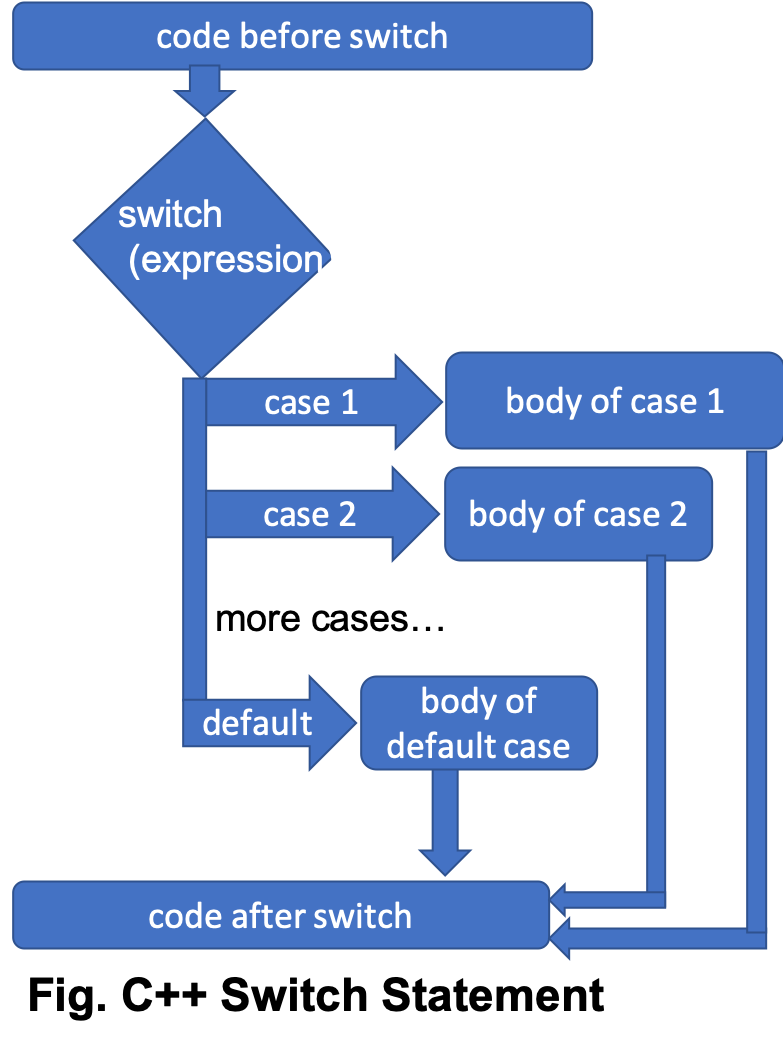
\includegraphics{resources/switch.png}

    \begin{tcolorbox}[breakable, size=fbox, boxrule=1pt, pad at break*=1mm,colback=cellbackground, colframe=cellborder]
\prompt{In}{incolor}{33}{\boxspacing}
\begin{Verbatim}[commandchars=\\\{\}]
\PY{c+c1}{// e.g. of a switch statement}
\PY{c+c1}{// determine name of the day given the number 1\PYZhy{}7}
\PY{k+kt}{unsigned} \PY{k+kt}{int} \PY{n}{day}\PY{p}{;}
\end{Verbatim}
\end{tcolorbox}

    \begin{tcolorbox}[breakable, size=fbox, boxrule=1pt, pad at break*=1mm,colback=cellbackground, colframe=cellborder]
\prompt{In}{incolor}{34}{\boxspacing}
\begin{Verbatim}[commandchars=\\\{\}]
\PY{n}{cout} \PY{o}{\PYZlt{}}\PY{o}{\PYZlt{}} \PY{l+s}{\PYZdq{}}\PY{l+s}{Enter day of the week 1\PYZhy{}7: }\PY{l+s}{\PYZdq{}}\PY{p}{;}
\PY{n}{cin} \PY{o}{\PYZgt{}}\PY{o}{\PYZgt{}} \PY{n}{day}\PY{p}{;}
\end{Verbatim}
\end{tcolorbox}

    \begin{Verbatim}[commandchars=\\\{\}]
Enter day of the week 1-7: 6
    \end{Verbatim}

    \begin{tcolorbox}[breakable, size=fbox, boxrule=1pt, pad at break*=1mm,colback=cellbackground, colframe=cellborder]
\prompt{In}{incolor}{35}{\boxspacing}
\begin{Verbatim}[commandchars=\\\{\}]
\PY{c+c1}{// comment out break; and see the result}
\PY{k}{switch}\PY{p}{(}\PY{n}{day}\PY{p}{)} \PY{p}{\PYZob{}}
    \PY{k}{case} \PY{l+m+mi}{1}\PY{o}{:} 
        \PY{n}{cout} \PY{o}{\PYZlt{}}\PY{o}{\PYZlt{}} \PY{l+s}{\PYZdq{}}\PY{l+s}{Day is Sunday}\PY{l+s+se}{\PYZbs{}n}\PY{l+s}{\PYZdq{}}\PY{p}{;}
        \PY{k}{break}\PY{p}{;}
    \PY{k}{case} \PY{l+m+mi}{2}\PY{o}{:}
        \PY{n}{cout} \PY{o}{\PYZlt{}}\PY{o}{\PYZlt{}} \PY{l+s}{\PYZdq{}}\PY{l+s}{Day is Monday}\PY{l+s+se}{\PYZbs{}n}\PY{l+s}{\PYZdq{}}\PY{p}{;}
        \PY{k}{break}\PY{p}{;}
    \PY{k}{case} \PY{l+m+mi}{3}\PY{o}{:}
        \PY{n}{cout} \PY{o}{\PYZlt{}}\PY{o}{\PYZlt{}} \PY{l+s}{\PYZdq{}}\PY{l+s}{Day is Tuesday}\PY{l+s+se}{\PYZbs{}n}\PY{l+s}{\PYZdq{}}\PY{p}{;}
        \PY{k}{break}\PY{p}{;}
    \PY{k}{case} \PY{l+m+mi}{4}\PY{o}{:}
        \PY{n}{cout} \PY{o}{\PYZlt{}}\PY{o}{\PYZlt{}} \PY{l+s}{\PYZdq{}}\PY{l+s}{Day is Wednesday}\PY{l+s+se}{\PYZbs{}n}\PY{l+s}{\PYZdq{}}\PY{p}{;}
        \PY{k}{break}\PY{p}{;}
    \PY{k}{case} \PY{l+m+mi}{5}\PY{o}{:}
        \PY{n}{cout} \PY{o}{\PYZlt{}}\PY{o}{\PYZlt{}} \PY{l+s}{\PYZdq{}}\PY{l+s}{Day is Thursday}\PY{l+s+se}{\PYZbs{}n}\PY{l+s}{\PYZdq{}}\PY{p}{;}
        \PY{k}{break}\PY{p}{;}
    \PY{k}{case} \PY{l+m+mi}{6}\PY{o}{:}
        \PY{n}{cout} \PY{o}{\PYZlt{}}\PY{o}{\PYZlt{}} \PY{l+s}{\PYZdq{}}\PY{l+s}{Day is Friday}\PY{l+s+se}{\PYZbs{}n}\PY{l+s}{\PYZdq{}}\PY{p}{;}
        \PY{k}{break}\PY{p}{;}
    \PY{k}{case} \PY{l+m+mi}{7}\PY{o}{:}
        \PY{n}{cout} \PY{o}{\PYZlt{}}\PY{o}{\PYZlt{}} \PY{l+s}{\PYZdq{}}\PY{l+s}{Day is Saturday}\PY{l+s+se}{\PYZbs{}n}\PY{l+s}{\PYZdq{}}\PY{p}{;}
        \PY{k}{break}\PY{p}{;}
    \PY{k}{default}\PY{o}{:}
        \PY{n}{cout} \PY{o}{\PYZlt{}}\PY{o}{\PYZlt{}} \PY{n}{day} \PY{o}{\PYZlt{}}\PY{o}{\PYZlt{}} \PY{l+s}{\PYZdq{}}\PY{l+s}{ is not a valid day!}\PY{l+s+se}{\PYZbs{}n}\PY{l+s}{\PYZdq{}}\PY{p}{;}
        \PY{c+c1}{//break; not required!}
\PY{p}{\PYZcb{}}
\end{Verbatim}
\end{tcolorbox}

    \begin{Verbatim}[commandchars=\\\{\}]
Day is Friday
    \end{Verbatim}

    \hypertarget{menu-driven-cli-interface}{%
\subsubsection{Menu-driven CLI
interface}\label{menu-driven-cli-interface}}

\begin{itemize}
\item
  command-line interface (CLI), though not as intuitive as Graphical
  User Interface (GUI), is still used widely
\item
  airline reservation systems, check-in and printing boarding passes,
  point-of-sale (POS) terminals at big companies such as Lowe's, Home
  Depot, etc. use CLI
\item
  a lot of text-based games used CLI as well
\item
  a good application of switch statement is in developing menu-driven
  CLI
\end{itemize}

\hypertarget{write-a-menu-driven-c-program-that-calculates-various-statistics-of-any-2-numbers}{%
\subsubsection{write a menu-driven C++ program that calculates various
statistics of any 2
numbers}\label{write-a-menu-driven-c-program-that-calculates-various-statistics-of-any-2-numbers}}

    \begin{tcolorbox}[breakable, size=fbox, boxrule=1pt, pad at break*=1mm,colback=cellbackground, colframe=cellborder]
\prompt{In}{incolor}{36}{\boxspacing}
\begin{Verbatim}[commandchars=\\\{\}]
\PY{c+cp}{\PYZsh{}}\PY{c+cp}{include} \PY{c+cpf}{\PYZlt{}iostream\PYZgt{}}
\PY{c+cp}{\PYZsh{}}\PY{c+cp}{include} \PY{c+cpf}{\PYZlt{}string\PYZgt{}}
\PY{c+cp}{\PYZsh{}}\PY{c+cp}{include} \PY{c+cpf}{\PYZlt{}cassert\PYZgt{}}
\PY{c+cp}{\PYZsh{}}\PY{c+cp}{include} \PY{c+cpf}{\PYZlt{}cmath\PYZgt{}}
\PY{c+cp}{\PYZsh{}}\PY{c+cp}{include} \PY{c+cpf}{\PYZlt{}iomanip\PYZgt{}}
\PY{c+cp}{\PYZsh{}}\PY{c+cp}{include} \PY{c+cpf}{\PYZlt{}sstream\PYZgt{}}

\PY{k}{using} \PY{k}{namespace} \PY{n+nn}{std}\PY{p}{;}
\end{Verbatim}
\end{tcolorbox}

    \begin{tcolorbox}[breakable, size=fbox, boxrule=1pt, pad at break*=1mm,colback=cellbackground, colframe=cellborder]
\prompt{In}{incolor}{37}{\boxspacing}
\begin{Verbatim}[commandchars=\\\{\}]
\PY{k}{template}\PY{o}{\PYZlt{}}\PY{k}{class} \PY{n+nc}{T}\PY{o}{\PYZgt{}}
\PY{n}{T} \PY{n}{add}\PY{p}{(}\PY{n}{T} \PY{n}{val1}\PY{p}{,} \PY{n}{T} \PY{n}{val2}\PY{p}{)} \PY{p}{\PYZob{}}
    \PY{k}{return} \PY{n}{val1} \PY{o}{+} \PY{n}{val2}\PY{p}{;}
\PY{p}{\PYZcb{}}
\end{Verbatim}
\end{tcolorbox}

    \begin{tcolorbox}[breakable, size=fbox, boxrule=1pt, pad at break*=1mm,colback=cellbackground, colframe=cellborder]
\prompt{In}{incolor}{38}{\boxspacing}
\begin{Verbatim}[commandchars=\\\{\}]
\PY{k}{template}\PY{o}{\PYZlt{}}\PY{k}{class} \PY{n+nc}{T}\PY{o}{\PYZgt{}}
\PY{n}{T} \PY{n}{subtract}\PY{p}{(}\PY{n}{T} \PY{n}{val1}\PY{p}{,} \PY{n}{T} \PY{n}{val2}\PY{p}{)} \PY{p}{\PYZob{}}
    \PY{k}{return} \PY{n}{val1} \PY{o}{\PYZhy{}} \PY{n}{val2}\PY{p}{;}
\PY{p}{\PYZcb{}}
\end{Verbatim}
\end{tcolorbox}

    \begin{tcolorbox}[breakable, size=fbox, boxrule=1pt, pad at break*=1mm,colback=cellbackground, colframe=cellborder]
\prompt{In}{incolor}{39}{\boxspacing}
\begin{Verbatim}[commandchars=\\\{\}]
\PY{k}{template}\PY{o}{\PYZlt{}}\PY{k}{class} \PY{n+nc}{T}\PY{o}{\PYZgt{}}
\PY{n}{T} \PY{n}{larger}\PY{p}{(}\PY{n}{T} \PY{n}{val1}\PY{p}{,} \PY{n}{T} \PY{n}{val2}\PY{p}{)} \PY{p}{\PYZob{}}
    \PY{k}{return} \PY{n}{val1} \PY{o}{\PYZgt{}}\PY{o}{=} \PY{n}{val2} \PY{o}{?} \PY{n+nl}{val1} \PY{p}{:} \PY{n}{val2}\PY{p}{;}
\PY{p}{\PYZcb{}}
\end{Verbatim}
\end{tcolorbox}

    \begin{tcolorbox}[breakable, size=fbox, boxrule=1pt, pad at break*=1mm,colback=cellbackground, colframe=cellborder]
\prompt{In}{incolor}{40}{\boxspacing}
\begin{Verbatim}[commandchars=\\\{\}]
\PY{k}{template}\PY{o}{\PYZlt{}}\PY{k}{class} \PY{n+nc}{T}\PY{o}{\PYZgt{}}
\PY{k+kt}{double} \PY{n}{average}\PY{p}{(}\PY{n}{T} \PY{n}{val1}\PY{p}{,} \PY{n}{T} \PY{n}{val2}\PY{p}{)} \PY{p}{\PYZob{}}
    \PY{k}{return} \PY{n}{add}\PY{p}{(}\PY{n}{val1}\PY{p}{,} \PY{n}{val2}\PY{p}{)}\PY{o}{/}\PY{l+m+mf}{2.0}\PY{p}{;}
\PY{p}{\PYZcb{}}
\end{Verbatim}
\end{tcolorbox}

    \begin{tcolorbox}[breakable, size=fbox, boxrule=1pt, pad at break*=1mm,colback=cellbackground, colframe=cellborder]
\prompt{In}{incolor}{41}{\boxspacing}
\begin{Verbatim}[commandchars=\\\{\}]
\PY{k+kt}{int} \PY{n+nf}{getMenuOption}\PY{p}{(}\PY{p}{)} \PY{p}{\PYZob{}}
    \PY{c+c1}{// A Smiple CLI\PYZhy{}based calculator}
    \PY{k+kt}{int} \PY{n}{option}\PY{p}{;}
    \PY{n}{cout} \PY{o}{\PYZlt{}}\PY{o}{\PYZlt{}} \PY{l+s}{\PYZdq{}}\PY{l+s}{Enter one of the following menu options: [1\PYZhy{}6]}\PY{l+s+se}{\PYZbs{}n}\PY{l+s}{\PYZdq{}}
        \PY{l+s}{\PYZdq{}}\PY{l+s}{1 \PYZhy{}\PYZgt{} Add}\PY{l+s+se}{\PYZbs{}n}\PY{l+s}{\PYZdq{}}
        \PY{o}{\PYZlt{}}\PY{o}{\PYZlt{}} \PY{l+s}{\PYZdq{}}\PY{l+s}{2 \PYZhy{}\PYZgt{} Subtract}\PY{l+s+se}{\PYZbs{}n}\PY{l+s}{\PYZdq{}}
        \PY{o}{\PYZlt{}}\PY{o}{\PYZlt{}} \PY{l+s}{\PYZdq{}}\PY{l+s}{3 \PYZhy{}\PYZgt{} Larger}\PY{l+s+se}{\PYZbs{}n}\PY{l+s}{\PYZdq{}}
        \PY{o}{\PYZlt{}}\PY{o}{\PYZlt{}} \PY{l+s}{\PYZdq{}}\PY{l+s}{4 \PYZhy{}\PYZgt{} Average}\PY{l+s+se}{\PYZbs{}n}\PY{l+s}{\PYZdq{}}
        \PY{o}{\PYZlt{}}\PY{o}{\PYZlt{}} \PY{l+s}{\PYZdq{}}\PY{l+s}{5 \PYZhy{}\PYZgt{} Multiply}\PY{l+s+se}{\PYZbs{}n}\PY{l+s}{\PYZdq{}}
        \PY{o}{\PYZlt{}}\PY{o}{\PYZlt{}} \PY{l+s}{\PYZdq{}}\PY{l+s}{6 \PYZhy{}\PYZgt{} Quit}\PY{l+s+se}{\PYZbs{}n}\PY{l+s}{\PYZdq{}}\PY{p}{;}
    \PY{n}{cin} \PY{o}{\PYZgt{}}\PY{o}{\PYZgt{}} \PY{n}{option}\PY{p}{;}
    \PY{k}{return} \PY{n}{option}\PY{p}{;}
\PY{p}{\PYZcb{}}
\end{Verbatim}
\end{tcolorbox}

    \begin{tcolorbox}[breakable, size=fbox, boxrule=1pt, pad at break*=1mm,colback=cellbackground, colframe=cellborder]
\prompt{In}{incolor}{42}{\boxspacing}
\begin{Verbatim}[commandchars=\\\{\}]
\PY{k+kt}{void} \PY{n+nf}{program}\PY{p}{(}\PY{p}{)} \PY{p}{\PYZob{}}
    \PY{k+kt}{float} \PY{n}{n1}\PY{p}{,} \PY{n}{n2}\PY{p}{;}
    \PY{k+kt}{int} \PY{n}{option}\PY{p}{;}
    \PY{n}{option} \PY{o}{=} \PY{n}{getMenuOption}\PY{p}{(}\PY{p}{)}\PY{p}{;}
    \PY{k}{if} \PY{p}{(}\PY{n}{option} \PY{o}{=}\PY{o}{=} \PY{l+m+mi}{6}\PY{p}{)} \PY{p}{\PYZob{}}
        \PY{n}{cout} \PY{o}{\PYZlt{}}\PY{o}{\PYZlt{}} \PY{l+s}{\PYZdq{}}\PY{l+s}{Good bye...}\PY{l+s+se}{\PYZbs{}n}\PY{l+s}{\PYZdq{}}\PY{p}{;}
        \PY{k}{return}\PY{p}{;}
    \PY{p}{\PYZcb{}}
    \PY{n}{cout} \PY{o}{\PYZlt{}}\PY{o}{\PYZlt{}} \PY{l+s}{\PYZdq{}}\PY{l+s}{Enter two numbers separated by space: }\PY{l+s}{\PYZdq{}}\PY{p}{;}
    \PY{n}{cin} \PY{o}{\PYZgt{}}\PY{o}{\PYZgt{}} \PY{n}{n1} \PY{o}{\PYZgt{}}\PY{o}{\PYZgt{}} \PY{n}{n2}\PY{p}{;}
    \PY{k}{switch}\PY{p}{(}\PY{n}{option}\PY{p}{)} \PY{p}{\PYZob{}}
        \PY{k}{case} \PY{l+m+mi}{1}\PY{o}{:}
            \PY{n}{cout} \PY{o}{\PYZlt{}}\PY{o}{\PYZlt{}} \PY{n}{n1} \PY{o}{\PYZlt{}}\PY{o}{\PYZlt{}} \PY{l+s}{\PYZdq{}}\PY{l+s}{ + }\PY{l+s}{\PYZdq{}} \PY{o}{\PYZlt{}}\PY{o}{\PYZlt{}} \PY{n}{n2} \PY{o}{\PYZlt{}}\PY{o}{\PYZlt{}} \PY{l+s}{\PYZdq{}}\PY{l+s}{ = }\PY{l+s}{\PYZdq{}} \PY{o}{\PYZlt{}}\PY{o}{\PYZlt{}} \PY{n}{add}\PY{o}{\PYZlt{}}\PY{k+kt}{float}\PY{o}{\PYZgt{}}\PY{p}{(}\PY{n}{n1}\PY{p}{,} \PY{n}{n2}\PY{p}{)} \PY{o}{\PYZlt{}}\PY{o}{\PYZlt{}} \PY{n}{endl}\PY{p}{;}
            \PY{k}{break}\PY{p}{;} \PY{c+c1}{// terminate switch}
        \PY{k}{case} \PY{l+m+mi}{2}\PY{o}{:}
            \PY{n}{cout} \PY{o}{\PYZlt{}}\PY{o}{\PYZlt{}} \PY{n}{n1} \PY{o}{\PYZlt{}}\PY{o}{\PYZlt{}} \PY{l+s}{\PYZdq{}}\PY{l+s}{ \PYZhy{} }\PY{l+s}{\PYZdq{}} \PY{o}{\PYZlt{}}\PY{o}{\PYZlt{}} \PY{n}{n2} \PY{o}{\PYZlt{}}\PY{o}{\PYZlt{}} \PY{l+s}{\PYZdq{}}\PY{l+s}{ = }\PY{l+s}{\PYZdq{}} \PY{o}{\PYZlt{}}\PY{o}{\PYZlt{}} \PY{n}{subtract}\PY{o}{\PYZlt{}}\PY{k+kt}{float}\PY{o}{\PYZgt{}}\PY{p}{(}\PY{n}{n1}\PY{p}{,} \PY{n}{n2}\PY{p}{)} \PY{o}{\PYZlt{}}\PY{o}{\PYZlt{}} \PY{n}{endl}\PY{p}{;}
            \PY{k}{break}\PY{p}{;}
        \PY{k}{case} \PY{l+m+mi}{3}\PY{o}{:}
            \PY{n}{cout} \PY{o}{\PYZlt{}}\PY{o}{\PYZlt{}} \PY{l+s}{\PYZdq{}}\PY{l+s}{larger between: }\PY{l+s}{\PYZdq{}} \PY{o}{\PYZlt{}}\PY{o}{\PYZlt{}} \PY{n}{n1} \PY{o}{\PYZlt{}}\PY{o}{\PYZlt{}} \PY{l+s}{\PYZdq{}}\PY{l+s}{ and }\PY{l+s}{\PYZdq{}} \PY{o}{\PYZlt{}}\PY{o}{\PYZlt{}} \PY{n}{n2} \PY{o}{\PYZlt{}}\PY{o}{\PYZlt{}} \PY{l+s}{\PYZdq{}}\PY{l+s}{ is }\PY{l+s}{\PYZdq{}} \PY{o}{\PYZlt{}}\PY{o}{\PYZlt{}} \PY{n}{larger}\PY{o}{\PYZlt{}}\PY{k+kt}{float}\PY{o}{\PYZgt{}}\PY{p}{(}\PY{n}{n1}\PY{p}{,} \PY{n}{n2}\PY{p}{)} \PY{o}{\PYZlt{}}\PY{o}{\PYZlt{}} \PY{n}{endl}\PY{p}{;}
            \PY{k}{break}\PY{p}{;}
        \PY{k}{case} \PY{l+m+mi}{4}\PY{o}{:}
            \PY{n}{cout} \PY{o}{\PYZlt{}}\PY{o}{\PYZlt{}} \PY{l+s}{\PYZdq{}}\PY{l+s}{average of }\PY{l+s}{\PYZdq{}} \PY{o}{\PYZlt{}}\PY{o}{\PYZlt{}} \PY{n}{n1} \PY{o}{\PYZlt{}}\PY{o}{\PYZlt{}} \PY{l+s}{\PYZdq{}}\PY{l+s}{ and }\PY{l+s}{\PYZdq{}} \PY{o}{\PYZlt{}}\PY{o}{\PYZlt{}} \PY{n}{n2} \PY{o}{\PYZlt{}}\PY{o}{\PYZlt{}} \PY{l+s}{\PYZdq{}}\PY{l+s}{ = }\PY{l+s}{\PYZdq{}} \PY{o}{\PYZlt{}}\PY{o}{\PYZlt{}} \PY{n}{average}\PY{o}{\PYZlt{}}\PY{k+kt}{float}\PY{o}{\PYZgt{}}\PY{p}{(}\PY{n}{n1}\PY{p}{,} \PY{n}{n2}\PY{p}{)} \PY{o}{\PYZlt{}}\PY{o}{\PYZlt{}} \PY{n}{endl}\PY{p}{;}
            \PY{k}{break}\PY{p}{;}
        \PY{k}{default}\PY{o}{:}
            \PY{n}{cout} \PY{o}{\PYZlt{}}\PY{o}{\PYZlt{}} \PY{n}{n1} \PY{o}{\PYZlt{}}\PY{o}{\PYZlt{}} \PY{l+s}{\PYZdq{}}\PY{l+s}{ x }\PY{l+s}{\PYZdq{}} \PY{o}{\PYZlt{}}\PY{o}{\PYZlt{}} \PY{n}{n2} \PY{o}{\PYZlt{}}\PY{o}{\PYZlt{}} \PY{l+s}{\PYZdq{}}\PY{l+s}{ = }\PY{l+s}{\PYZdq{}} \PY{o}{\PYZlt{}}\PY{o}{\PYZlt{}} \PY{n}{n1}\PY{o}{*}\PY{n}{n2} \PY{o}{\PYZlt{}}\PY{o}{\PYZlt{}} \PY{n}{endl}\PY{p}{;}
            \PY{k}{break}\PY{p}{;}
    \PY{p}{\PYZcb{}}
\PY{p}{\PYZcb{}}
\end{Verbatim}
\end{tcolorbox}

    \begin{tcolorbox}[breakable, size=fbox, boxrule=1pt, pad at break*=1mm,colback=cellbackground, colframe=cellborder]
\prompt{In}{incolor}{43}{\boxspacing}
\begin{Verbatim}[commandchars=\\\{\}]
\PY{c+c1}{// TODO: run this many times...}
\PY{n}{program}\PY{p}{(}\PY{p}{)}\PY{p}{;}
\end{Verbatim}
\end{tcolorbox}

    \begin{Verbatim}[commandchars=\\\{\}]
Enter one of the following menu options: [1-6]
1 -> Add
2 -> Subtract
3 -> Larger
4 -> Average
5 -> Multiply
6 -> Quit
1
Enter two numbers separated by space: 3 105
3 + 105 = 108
    \end{Verbatim}

    \hypertarget{note-a-loop-would-work-better-for-menu-driven-program}{%
\subsubsection{Note: a loop would work better for menu-driven
program}\label{note-a-loop-would-work-better-for-menu-driven-program}}

\begin{itemize}
\tightlist
\item
  loop is covered in next chapter
\end{itemize}

\hypertarget{a-complete-demo-program-is-here-demosconditionalsmenumenu.cpp}{%
\subsubsection{\texorpdfstring{A complete demo program is here:
\url{demos/conditionals/menu/menu.cpp}}{A complete demo program is here: demos/conditionals/menu/menu.cpp}}\label{a-complete-demo-program-is-here-demosconditionalsmenumenu.cpp}}

\hypertarget{rectangle-demo-program-demosconditionalsrectanglemain.cpp}{%
\subsubsection{\texorpdfstring{Rectangle demo program
\url{demos/conditionals/rectangle/main.cpp}}{Rectangle demo program demos/conditionals/rectangle/main.cpp}}\label{rectangle-demo-program-demosconditionalsrectanglemain.cpp}}

\begin{itemize}
\tightlist
\item
  An improvded Rectangle program from previous chapter that calls
  automated test when user wants to by passing argument to the main
\end{itemize}

    \hypertarget{exercises}{%
\subsection{Exercises}\label{exercises}}

\begin{enumerate}
\def\labelenumi{\arabic{enumi}.}
\item
  Write a program that helps someone decide where to go eat lunch
  depending on amount of money one has in their pocket.
\item
  Improve exercise 1 by using function(s) and writing at least 3 test
  cases for each function.
\item
  Write a program that determines whether someone is eligible to vote in
  the US federal election.

  \begin{itemize}
  \tightlist
  \item
    see sample solution here
    \url{exercises/conditionals/vote1/voting_eligibility.cpp}
  \end{itemize}
\item
  Improve exercise 3 by using function(s) and writing at least 3 test
  cases for each function.

  \begin{itemize}
  \tightlist
  \item
    see sample solution here
    \url{exercises/conditionals/vote2/voting_eligibility_v2.cpp}
  \end{itemize}
\item
  Write a function day\_name that converts an integer number 0 to 6 into
  the name of a day. Assume day 0 is ``Sunday''. Return ``Invalid Day''
  if the argument to the function is not valid.
\end{enumerate}

    \begin{tcolorbox}[breakable, size=fbox, boxrule=1pt, pad at break*=1mm,colback=cellbackground, colframe=cellborder]
\prompt{In}{incolor}{45}{\boxspacing}
\begin{Verbatim}[commandchars=\\\{\}]
\PY{c+c1}{// code stub for Exercise 5}
\PY{n}{string} \PY{n+nf}{day\PYZus{}name}\PY{p}{(}\PY{k+kt}{int} \PY{n}{day}\PY{p}{)} \PY{p}{\PYZob{}}
    \PY{c+c1}{// FIXME \PYZhy{} complete the rest}
    \PY{k}{return} \PY{l+s}{\PYZdq{}}\PY{l+s}{\PYZdq{}}\PY{p}{;}
\PY{p}{\PYZcb{}}
\end{Verbatim}
\end{tcolorbox}

    \begin{tcolorbox}[breakable, size=fbox, boxrule=1pt, pad at break*=1mm,colback=cellbackground, colframe=cellborder]
\prompt{In}{incolor}{ }{\boxspacing}
\begin{Verbatim}[commandchars=\\\{\}]
\PY{c+c1}{// Here are some tests that should pass for day\PYZus{}name function defined above}
\PY{k+kt}{void} \PY{n+nf}{test\PYZus{}day\PYZus{}name}\PY{p}{(}\PY{p}{)} \PY{p}{\PYZob{}}
    \PY{n}{assert}\PY{p}{(}\PY{n}{day\PYZus{}name}\PY{p}{(}\PY{l+m+mi}{3}\PY{p}{)} \PY{o}{=}\PY{o}{=} \PY{l+s}{\PYZdq{}}\PY{l+s}{Wednesday}\PY{l+s}{\PYZdq{}}\PY{p}{)}\PY{p}{;}
    \PY{n}{assert}\PY{p}{(}\PY{n}{day\PYZus{}name}\PY{p}{(}\PY{l+m+mi}{6}\PY{p}{)} \PY{o}{=}\PY{o}{=} \PY{l+s}{\PYZdq{}}\PY{l+s}{Saturday}\PY{l+s}{\PYZdq{}}\PY{p}{)}\PY{p}{;}
    \PY{n}{assert}\PY{p}{(}\PY{n}{day\PYZus{}name}\PY{p}{(}\PY{l+m+mi}{42}\PY{p}{)} \PY{o}{=}\PY{o}{=} \PY{l+s}{\PYZdq{}}\PY{l+s}{Invalid Day}\PY{l+s}{\PYZdq{}}\PY{p}{)}\PY{p}{;}
    \PY{n}{cout} \PY{o}{\PYZlt{}}\PY{o}{\PYZlt{}} \PY{l+s}{\PYZdq{}}\PY{l+s}{all test cases passed for day\PYZus{}name()}\PY{l+s+se}{\PYZbs{}n}\PY{l+s}{\PYZdq{}}\PY{p}{;}
\PY{p}{\PYZcb{}}
\end{Verbatim}
\end{tcolorbox}

    \begin{enumerate}
\def\labelenumi{\arabic{enumi}.}
\setcounter{enumi}{5}
\tightlist
\item
  Improve exercise 5 as a complete program with algorithm stepts,
  main(), etc.
\end{enumerate}

    \begin{enumerate}
\def\labelenumi{\arabic{enumi}.}
\setcounter{enumi}{6}
\tightlist
\item
  Write a function that helps answer questions like ``Today is
  Wednesday. I leave on holiday in 19 days time. What day will that
  be?'' So, the function must take a day name and a delta argument (the
  number of days to add) and should return the resulting day name.
\end{enumerate}

    \begin{tcolorbox}[breakable, size=fbox, boxrule=1pt, pad at break*=1mm,colback=cellbackground, colframe=cellborder]
\prompt{In}{incolor}{ }{\boxspacing}
\begin{Verbatim}[commandchars=\\\{\}]
\PY{c+c1}{// Exercise 6 hints}
\PY{n}{string} \PY{n+nf}{day\PYZus{}add}\PY{p}{(}\PY{n}{string} \PY{n}{dayName}\PY{p}{,} \PY{k+kt}{int} \PY{n}{delta}\PY{p}{)} \PY{p}{\PYZob{}}
    \PY{c+c1}{// FIXME}
\PY{p}{\PYZcb{}}
\end{Verbatim}
\end{tcolorbox}

    \begin{tcolorbox}[breakable, size=fbox, boxrule=1pt, pad at break*=1mm,colback=cellbackground, colframe=cellborder]
\prompt{In}{incolor}{ }{\boxspacing}
\begin{Verbatim}[commandchars=\\\{\}]
\PY{c+c1}{// Exercise 6 test function}
\PY{c+c1}{// here are some tests that should pass}
\PY{k+kt}{void} \PY{n+nf}{test\PYZus{}day\PYZus{}add}\PY{p}{(}\PY{p}{)} \PY{p}{\PYZob{}}
    \PY{n}{assert}\PY{p}{(}\PY{n}{day\PYZus{}add}\PY{p}{(}\PY{l+s}{\PYZdq{}}\PY{l+s}{Monday}\PY{l+s}{\PYZdq{}}\PY{p}{,} \PY{l+m+mi}{4}\PY{p}{)} \PY{o}{=}\PY{o}{=}  \PY{l+s}{\PYZdq{}}\PY{l+s}{Friday}\PY{l+s}{\PYZdq{}}\PY{p}{)}\PY{p}{;}
    \PY{n}{assert}\PY{p}{(}\PY{n}{day\PYZus{}add}\PY{p}{(}\PY{l+s}{\PYZdq{}}\PY{l+s}{Tuesday}\PY{l+s}{\PYZdq{}}\PY{p}{,} \PY{l+m+mi}{0}\PY{p}{)} \PY{o}{=}\PY{o}{=} \PY{l+s}{\PYZdq{}}\PY{l+s}{Tuesday}\PY{l+s}{\PYZdq{}}\PY{p}{)}\PY{p}{;}
    \PY{n}{assert}\PY{p}{(}\PY{n}{day\PYZus{}add}\PY{p}{(}\PY{l+s}{\PYZdq{}}\PY{l+s}{Tuesday}\PY{l+s}{\PYZdq{}}\PY{p}{,} \PY{l+m+mi}{14}\PY{p}{)} \PY{o}{=}\PY{o}{=} \PY{l+s}{\PYZdq{}}\PY{l+s}{Tuesday}\PY{l+s}{\PYZdq{}}\PY{p}{)}\PY{p}{;}
    \PY{n}{assert}\PY{p}{(}\PY{n}{day\PYZus{}add}\PY{p}{(}\PY{l+s}{\PYZdq{}}\PY{l+s}{Sunday}\PY{l+s}{\PYZdq{}}\PY{p}{,} \PY{l+m+mi}{100}\PY{p}{)} \PY{o}{=}\PY{o}{=} \PY{l+s}{\PYZdq{}}\PY{l+s}{Tuesday}\PY{l+s}{\PYZdq{}}\PY{p}{)}\PY{p}{;}
    \PY{n}{assert}\PY{p}{(}\PY{n}{day\PYZus{}add}\PY{p}{(}\PY{l+s}{\PYZdq{}}\PY{l+s}{Sunday}\PY{l+s}{\PYZdq{}}\PY{p}{,} \PY{l+m+mi}{\PYZhy{}1}\PY{p}{)} \PY{o}{=}\PY{o}{=} \PY{l+s}{\PYZdq{}}\PY{l+s}{Saturday}\PY{l+s}{\PYZdq{}}\PY{p}{)}\PY{p}{;}
    \PY{n}{assert}\PY{p}{(}\PY{n}{day\PYZus{}add}\PY{p}{(}\PY{l+s}{\PYZdq{}}\PY{l+s}{Sunday}\PY{l+s}{\PYZdq{}}\PY{p}{,} \PY{l+m+mi}{\PYZhy{}7}\PY{p}{)} \PY{o}{=}\PY{o}{=} \PY{l+s}{\PYZdq{}}\PY{l+s}{Sunday}\PY{l+s}{\PYZdq{}}\PY{p}{)}\PY{p}{;}
    \PY{n}{assert}\PY{p}{(}\PY{n}{day\PYZus{}add}\PY{p}{(}\PY{l+s}{\PYZdq{}}\PY{l+s}{Tuesday}\PY{l+s}{\PYZdq{}}\PY{p}{,} \PY{l+m+mi}{\PYZhy{}100}\PY{p}{)} \PY{o}{=}\PY{o}{=} \PY{l+s}{\PYZdq{}}\PY{l+s}{Sunday}\PY{l+s}{\PYZdq{}}\PY{p}{)}\PY{p}{;}
    \PY{n}{cout} \PY{o}{\PYZlt{}}\PY{o}{\PYZlt{}} \PY{l+s}{\PYZdq{}}\PY{l+s}{all test cases passed for day\PYZus{}add()}\PY{l+s}{\PYZdq{}}\PY{p}{;}
\PY{p}{\PYZcb{}}
\end{Verbatim}
\end{tcolorbox}

    \begin{enumerate}
\def\labelenumi{\arabic{enumi}.}
\setcounter{enumi}{7}
\item
  Improve Exercise 7 as a complete program with algorithm steps, main(),
  etc.
\item
  Write a C++ program including algorithm steps that calculates area and
  perimeter of a triangle given three sides.

  \begin{itemize}
  \tightlist
  \item
    must define and use separate functions to calculate area and
    perimeter
  \item
    write at least 3 test cases for each function
  \item
    Hint: use Heron's formula to find area with three sides.
  \item
    define and use function to determine if 3 sides form a triangle
  \end{itemize}
\item
  Write a C++ program including algorithm steps that calculates Body
  Mass Index (BMI) of a person.

  \begin{itemize}
  \tightlist
  \item
    must use as many functions as possible
  \item
    write at least 3 test cases for each function
  \item
    more info on BMI -
    https://www.nhlbi.nih.gov/health/educational/lose\_wt/BMI/bmicalc.htm
  \item
    Formula
    \href{https://www.cdc.gov/healthyweight/assessing/bmi/childrens_bmi/childrens_bmi_formula.html\#:~:text=The\%20formula\%20for\%20BMI\%20is,to\%20convert\%20this\%20to\%20meters.\&text=When\%20using\%20English\%20measurements\%2C\%20pounds\%20should\%20be\%20divided\%20by\%20inches\%20squared}{here}.
  \item
    a sample solution is provided at
    \url{exercises/conditionals/BMI/BMI_v3.cpp}

    \begin{itemize}
    \tightlist
    \item
      \textbf{an improved version that interprets the BMI result}
    \end{itemize}
  \end{itemize}
\end{enumerate}

    \hypertarget{kattis-problems}{%
\subsection{Kattis Problems}\label{kattis-problems}}

\begin{itemize}
\tightlist
\item
  almost all Kattis problems require conditional statements
\item
  following are some problems that can be solved based on the concepts
  learned from Ch1-6
\item
  solve each problem using function(s)
\item
  write at least 3 test cases for each function
\end{itemize}

\begin{enumerate}
\def\labelenumi{\arabic{enumi}.}
\tightlist
\item
  Take Two Stones - https://open.kattis.com/problems/twostones

  \begin{itemize}
  \tightlist
  \item
    Hint: check even or odd
  \end{itemize}
\item
  Laptop Sticker - https://open.kattis.com/problems/laptopsticker

  \begin{itemize}
  \tightlist
  \item
    Hint: basic math
  \end{itemize}
\item
  Sort Two Numbers - https://open.kattis.com/problems/sorttwonumbers

  \begin{itemize}
  \tightlist
  \item
    Hint: compare two numbers and print their order
  \end{itemize}
\item
  FYI - https://open.kattis.com/problems/fyi

  \begin{itemize}
  \tightlist
  \item
    Hint: string.find() and condition
  \end{itemize}
\end{enumerate}

    \hypertarget{summary}{%
\subsection{Summary}\label{summary}}

\begin{itemize}
\tightlist
\item
  we learned about another fundamental concepts: conditional execution
\item
  learned with examples 3 different types of conditional statements
\item
  learned how to use conditional statements in functions
\item
  learned about ternary conditional operator (condition) ? exp1 : exp2

  \begin{itemize}
  \tightlist
  \item
    a short cut for alternative execution
  \end{itemize}
\item
  learned about comparision and logical operators; order of precedence
\item
  learned passing and using arguments to main( )
\item
  finally, exercise and sample solutions
\end{itemize}

    \begin{tcolorbox}[breakable, size=fbox, boxrule=1pt, pad at break*=1mm,colback=cellbackground, colframe=cellborder]
\prompt{In}{incolor}{ }{\boxspacing}
\begin{Verbatim}[commandchars=\\\{\}]

\end{Verbatim}
\end{tcolorbox}


    % Add a bibliography block to the postdoc
    
    
    
\end{document}
